


% Header, overrides base

    % Make sure that the sphinx doc style knows who it inherits from.
    \def\sphinxdocclass{article}

    % Declare the document class
    \documentclass[letterpaper,10pt,english]{/usr/share/sphinx/texinputs/sphinxhowto}

    % Imports
    \usepackage[utf8]{inputenc}
    \DeclareUnicodeCharacter{00A0}{\\nobreakspace}
    \usepackage[T1]{fontenc}
    \usepackage{babel}
    \usepackage{times}
    \usepackage{import}
    \usepackage[Bjarne]{/usr/share/sphinx/texinputs/fncychap}
    \usepackage{longtable}
    \usepackage{/usr/share/sphinx/texinputs/sphinx}
    \usepackage{multirow}

    \usepackage{amsmath}
    \usepackage{amssymb}
    \usepackage{ucs}
    \usepackage{enumerate}

    % Used to make the Input/Output rules follow around the contents.
    \usepackage{needspace}

    % Pygments requirements
    \usepackage{fancyvrb}
    \usepackage{color}
    % ansi colors additions
    \definecolor{darkgreen}{rgb}{.12,.54,.11}
    \definecolor{lightgray}{gray}{.95}
    \definecolor{brown}{rgb}{0.54,0.27,0.07}
    \definecolor{purple}{rgb}{0.5,0.0,0.5}
    \definecolor{darkgray}{gray}{0.25}
    \definecolor{lightred}{rgb}{1.0,0.39,0.28}
    \definecolor{lightgreen}{rgb}{0.48,0.99,0.0}
    \definecolor{lightblue}{rgb}{0.53,0.81,0.92}
    \definecolor{lightpurple}{rgb}{0.87,0.63,0.87}
    \definecolor{lightcyan}{rgb}{0.5,1.0,0.83}

    % Needed to box output/input
    \usepackage{tikz}
        \usetikzlibrary{calc,arrows,shadows}
    \usepackage[framemethod=tikz]{mdframed}

    \usepackage{alltt}

    % Used to load and display graphics
    \usepackage{graphicx}
    \graphicspath{ {figs/} }
    \usepackage[Export]{adjustbox} % To resize

    % used so that images for notebooks which have spaces in the name can still be included
    \usepackage{grffile}

    \usepackage[colorlinks]{hyperref}
    \usepackage{cleveref}

    % For formatting output while also word wrapping.
    \usepackage{listings}
    \lstset{breaklines=true}
    \lstset{basicstyle=\small\ttfamily}
    \def\smaller{\fontsize{9.5pt}{9.5pt}\selectfont}

    %Pygments definitions
    
\makeatletter
\def\PY@reset{\let\PY@it=\relax \let\PY@bf=\relax%
    \let\PY@ul=\relax \let\PY@tc=\relax%
    \let\PY@bc=\relax \let\PY@ff=\relax}
\def\PY@tok#1{\csname PY@tok@#1\endcsname}
\def\PY@toks#1+{\ifx\relax#1\empty\else%
    \PY@tok{#1}\expandafter\PY@toks\fi}
\def\PY@do#1{\PY@bc{\PY@tc{\PY@ul{%
    \PY@it{\PY@bf{\PY@ff{#1}}}}}}}
\def\PY#1#2{\PY@reset\PY@toks#1+\relax+\PY@do{#2}}

\expandafter\def\csname PY@tok@gd\endcsname{\def\PY@tc##1{\textcolor[rgb]{0.63,0.00,0.00}{##1}}}
\expandafter\def\csname PY@tok@gu\endcsname{\let\PY@bf=\textbf\def\PY@tc##1{\textcolor[rgb]{0.50,0.00,0.50}{##1}}}
\expandafter\def\csname PY@tok@gt\endcsname{\def\PY@tc##1{\textcolor[rgb]{0.00,0.27,0.87}{##1}}}
\expandafter\def\csname PY@tok@gs\endcsname{\let\PY@bf=\textbf}
\expandafter\def\csname PY@tok@gr\endcsname{\def\PY@tc##1{\textcolor[rgb]{1.00,0.00,0.00}{##1}}}
\expandafter\def\csname PY@tok@cm\endcsname{\let\PY@it=\textit\def\PY@tc##1{\textcolor[rgb]{0.25,0.50,0.50}{##1}}}
\expandafter\def\csname PY@tok@vg\endcsname{\def\PY@tc##1{\textcolor[rgb]{0.10,0.09,0.49}{##1}}}
\expandafter\def\csname PY@tok@m\endcsname{\def\PY@tc##1{\textcolor[rgb]{0.40,0.40,0.40}{##1}}}
\expandafter\def\csname PY@tok@mh\endcsname{\def\PY@tc##1{\textcolor[rgb]{0.40,0.40,0.40}{##1}}}
\expandafter\def\csname PY@tok@go\endcsname{\def\PY@tc##1{\textcolor[rgb]{0.53,0.53,0.53}{##1}}}
\expandafter\def\csname PY@tok@ge\endcsname{\let\PY@it=\textit}
\expandafter\def\csname PY@tok@vc\endcsname{\def\PY@tc##1{\textcolor[rgb]{0.10,0.09,0.49}{##1}}}
\expandafter\def\csname PY@tok@il\endcsname{\def\PY@tc##1{\textcolor[rgb]{0.40,0.40,0.40}{##1}}}
\expandafter\def\csname PY@tok@cs\endcsname{\let\PY@it=\textit\def\PY@tc##1{\textcolor[rgb]{0.25,0.50,0.50}{##1}}}
\expandafter\def\csname PY@tok@cp\endcsname{\def\PY@tc##1{\textcolor[rgb]{0.74,0.48,0.00}{##1}}}
\expandafter\def\csname PY@tok@gi\endcsname{\def\PY@tc##1{\textcolor[rgb]{0.00,0.63,0.00}{##1}}}
\expandafter\def\csname PY@tok@gh\endcsname{\let\PY@bf=\textbf\def\PY@tc##1{\textcolor[rgb]{0.00,0.00,0.50}{##1}}}
\expandafter\def\csname PY@tok@ni\endcsname{\let\PY@bf=\textbf\def\PY@tc##1{\textcolor[rgb]{0.60,0.60,0.60}{##1}}}
\expandafter\def\csname PY@tok@nl\endcsname{\def\PY@tc##1{\textcolor[rgb]{0.63,0.63,0.00}{##1}}}
\expandafter\def\csname PY@tok@nn\endcsname{\let\PY@bf=\textbf\def\PY@tc##1{\textcolor[rgb]{0.00,0.00,1.00}{##1}}}
\expandafter\def\csname PY@tok@no\endcsname{\def\PY@tc##1{\textcolor[rgb]{0.53,0.00,0.00}{##1}}}
\expandafter\def\csname PY@tok@na\endcsname{\def\PY@tc##1{\textcolor[rgb]{0.49,0.56,0.16}{##1}}}
\expandafter\def\csname PY@tok@nb\endcsname{\def\PY@tc##1{\textcolor[rgb]{0.00,0.50,0.00}{##1}}}
\expandafter\def\csname PY@tok@nc\endcsname{\let\PY@bf=\textbf\def\PY@tc##1{\textcolor[rgb]{0.00,0.00,1.00}{##1}}}
\expandafter\def\csname PY@tok@nd\endcsname{\def\PY@tc##1{\textcolor[rgb]{0.67,0.13,1.00}{##1}}}
\expandafter\def\csname PY@tok@ne\endcsname{\let\PY@bf=\textbf\def\PY@tc##1{\textcolor[rgb]{0.82,0.25,0.23}{##1}}}
\expandafter\def\csname PY@tok@nf\endcsname{\def\PY@tc##1{\textcolor[rgb]{0.00,0.00,1.00}{##1}}}
\expandafter\def\csname PY@tok@si\endcsname{\let\PY@bf=\textbf\def\PY@tc##1{\textcolor[rgb]{0.73,0.40,0.53}{##1}}}
\expandafter\def\csname PY@tok@s2\endcsname{\def\PY@tc##1{\textcolor[rgb]{0.73,0.13,0.13}{##1}}}
\expandafter\def\csname PY@tok@vi\endcsname{\def\PY@tc##1{\textcolor[rgb]{0.10,0.09,0.49}{##1}}}
\expandafter\def\csname PY@tok@nt\endcsname{\let\PY@bf=\textbf\def\PY@tc##1{\textcolor[rgb]{0.00,0.50,0.00}{##1}}}
\expandafter\def\csname PY@tok@nv\endcsname{\def\PY@tc##1{\textcolor[rgb]{0.10,0.09,0.49}{##1}}}
\expandafter\def\csname PY@tok@s1\endcsname{\def\PY@tc##1{\textcolor[rgb]{0.73,0.13,0.13}{##1}}}
\expandafter\def\csname PY@tok@sh\endcsname{\def\PY@tc##1{\textcolor[rgb]{0.73,0.13,0.13}{##1}}}
\expandafter\def\csname PY@tok@sc\endcsname{\def\PY@tc##1{\textcolor[rgb]{0.73,0.13,0.13}{##1}}}
\expandafter\def\csname PY@tok@sx\endcsname{\def\PY@tc##1{\textcolor[rgb]{0.00,0.50,0.00}{##1}}}
\expandafter\def\csname PY@tok@bp\endcsname{\def\PY@tc##1{\textcolor[rgb]{0.00,0.50,0.00}{##1}}}
\expandafter\def\csname PY@tok@c1\endcsname{\let\PY@it=\textit\def\PY@tc##1{\textcolor[rgb]{0.25,0.50,0.50}{##1}}}
\expandafter\def\csname PY@tok@kc\endcsname{\let\PY@bf=\textbf\def\PY@tc##1{\textcolor[rgb]{0.00,0.50,0.00}{##1}}}
\expandafter\def\csname PY@tok@c\endcsname{\let\PY@it=\textit\def\PY@tc##1{\textcolor[rgb]{0.25,0.50,0.50}{##1}}}
\expandafter\def\csname PY@tok@mf\endcsname{\def\PY@tc##1{\textcolor[rgb]{0.40,0.40,0.40}{##1}}}
\expandafter\def\csname PY@tok@err\endcsname{\def\PY@bc##1{\setlength{\fboxsep}{0pt}\fcolorbox[rgb]{1.00,0.00,0.00}{1,1,1}{\strut ##1}}}
\expandafter\def\csname PY@tok@kd\endcsname{\let\PY@bf=\textbf\def\PY@tc##1{\textcolor[rgb]{0.00,0.50,0.00}{##1}}}
\expandafter\def\csname PY@tok@ss\endcsname{\def\PY@tc##1{\textcolor[rgb]{0.10,0.09,0.49}{##1}}}
\expandafter\def\csname PY@tok@sr\endcsname{\def\PY@tc##1{\textcolor[rgb]{0.73,0.40,0.53}{##1}}}
\expandafter\def\csname PY@tok@mo\endcsname{\def\PY@tc##1{\textcolor[rgb]{0.40,0.40,0.40}{##1}}}
\expandafter\def\csname PY@tok@kn\endcsname{\let\PY@bf=\textbf\def\PY@tc##1{\textcolor[rgb]{0.00,0.50,0.00}{##1}}}
\expandafter\def\csname PY@tok@mi\endcsname{\def\PY@tc##1{\textcolor[rgb]{0.40,0.40,0.40}{##1}}}
\expandafter\def\csname PY@tok@gp\endcsname{\let\PY@bf=\textbf\def\PY@tc##1{\textcolor[rgb]{0.00,0.00,0.50}{##1}}}
\expandafter\def\csname PY@tok@o\endcsname{\def\PY@tc##1{\textcolor[rgb]{0.40,0.40,0.40}{##1}}}
\expandafter\def\csname PY@tok@kr\endcsname{\let\PY@bf=\textbf\def\PY@tc##1{\textcolor[rgb]{0.00,0.50,0.00}{##1}}}
\expandafter\def\csname PY@tok@s\endcsname{\def\PY@tc##1{\textcolor[rgb]{0.73,0.13,0.13}{##1}}}
\expandafter\def\csname PY@tok@kp\endcsname{\def\PY@tc##1{\textcolor[rgb]{0.00,0.50,0.00}{##1}}}
\expandafter\def\csname PY@tok@w\endcsname{\def\PY@tc##1{\textcolor[rgb]{0.73,0.73,0.73}{##1}}}
\expandafter\def\csname PY@tok@kt\endcsname{\def\PY@tc##1{\textcolor[rgb]{0.69,0.00,0.25}{##1}}}
\expandafter\def\csname PY@tok@ow\endcsname{\let\PY@bf=\textbf\def\PY@tc##1{\textcolor[rgb]{0.67,0.13,1.00}{##1}}}
\expandafter\def\csname PY@tok@sb\endcsname{\def\PY@tc##1{\textcolor[rgb]{0.73,0.13,0.13}{##1}}}
\expandafter\def\csname PY@tok@k\endcsname{\let\PY@bf=\textbf\def\PY@tc##1{\textcolor[rgb]{0.00,0.50,0.00}{##1}}}
\expandafter\def\csname PY@tok@se\endcsname{\let\PY@bf=\textbf\def\PY@tc##1{\textcolor[rgb]{0.73,0.40,0.13}{##1}}}
\expandafter\def\csname PY@tok@sd\endcsname{\let\PY@it=\textit\def\PY@tc##1{\textcolor[rgb]{0.73,0.13,0.13}{##1}}}

\def\PYZbs{\char`\\}
\def\PYZus{\char`\_}
\def\PYZob{\char`\{}
\def\PYZcb{\char`\}}
\def\PYZca{\char`\^}
\def\PYZam{\char`\&}
\def\PYZlt{\char`\<}
\def\PYZgt{\char`\>}
\def\PYZsh{\char`\#}
\def\PYZpc{\char`\%}
\def\PYZdl{\char`\$}
\def\PYZhy{\char`\-}
\def\PYZsq{\char`\'}
\def\PYZdq{\char`\"}
\def\PYZti{\char`\~}
% for compatibility with earlier versions
\def\PYZat{@}
\def\PYZlb{[}
\def\PYZrb{]}
\makeatother


    %Set pygments styles if needed...
    
        \definecolor{nbframe-border}{rgb}{0.867,0.867,0.867}
        \definecolor{nbframe-bg}{rgb}{0.969,0.969,0.969}
        \definecolor{nbframe-in-prompt}{rgb}{0.0,0.0,0.502}
        \definecolor{nbframe-out-prompt}{rgb}{0.545,0.0,0.0}

        \newenvironment{ColorVerbatim}
        {\begin{mdframed}[%
            roundcorner=1.0pt, %
            backgroundcolor=nbframe-bg, %
            userdefinedwidth=1\linewidth, %
            leftmargin=0.1\linewidth, %
            innerleftmargin=0pt, %
            innerrightmargin=0pt, %
            linecolor=nbframe-border, %
            linewidth=1pt, %
            usetwoside=false, %
            everyline=true, %
            innerlinewidth=3pt, %
            innerlinecolor=nbframe-bg, %
            middlelinewidth=1pt, %
            middlelinecolor=nbframe-bg, %
            outerlinewidth=0.5pt, %
            outerlinecolor=nbframe-border, %
            needspace=0pt
        ]}
        {\end{mdframed}}
        
        \newenvironment{InvisibleVerbatim}
        {\begin{mdframed}[leftmargin=0.1\linewidth,innerleftmargin=3pt,innerrightmargin=3pt, userdefinedwidth=1\linewidth, linewidth=0pt, linecolor=white, usetwoside=false]}
        {\end{mdframed}}

        \renewenvironment{Verbatim}[1][\unskip]
        {\begin{alltt}\smaller}
        {\end{alltt}}
    

    % Help prevent overflowing lines due to urls and other hard-to-break 
    % entities.  This doesn't catch everything...
    \sloppy

    % Document level variables
    \title{SCTDA Tutorial}
    \date{July 16, 2015}
    \release{}
    \author{Pablo G. C\'amara}
    \renewcommand{\releasename}{}

    % TODO: Add option for the user to specify a logo for his/her export.
    \newcommand{\sphinxlogo}{}

    % Make the index page of the document.
    \makeindex

    % Import sphinx document type specifics.
     


% Body

    % Start of the document
    \begin{document}

        
            \maketitle
        

        


        
SCTDA is an object oriented python library for topological data analysis of
high-throughput single-cell RNA-seq data. It includes tools
for the preprocessing, analysis and exploration of single-cell RNA-seq data,
based on condensed topological representations produced by software such
as \href{http://danifold.net/mapper/}{Mapper} or \href{http://www.ayasdi.com/}{Ayasdi}. This tutorial illustrates the basic SCTDA workflow using the motor neuron dataset of \cite{ref1} as case study. It is based on an IPython notebook.

    % Make sure that atleast 4 lines are below the HR
    \needspace{4\baselineskip}

    
        \vspace{8pt}
        \makebox[0.1\linewidth]{\smaller\hfill\tt\color{nbframe-in-prompt}In\hspace{4pt}{[}1{]}:\hspace{4pt}}\\*
        \vspace{-2.1\baselineskip}
        \begin{ColorVerbatim}
            \vspace{-0.2\baselineskip}
            \begin{Verbatim}[commandchars=\\\{\}]
\PY{k+kn}{import} \PY{n+nn}{SCTDA}
\end{Verbatim}

            
                \vspace{-0.2\baselineskip}
            
        \end{ColorVerbatim}
    
\section{Preliminary steps}

\subsection{Pre-processing}

For convenience, SCTDA includes a class for preparing and filtering single-cell expression data,
based on RNA spike-in read counts. It takes as input one or more files with read
counts in the format of \href{http://www-huber.embl.de/users/anders/HTSeq/doc/overview.html}{HTSeq-count}. Files can be all from a same time
point or from multiple time points of a continuous biological process. In this tutorial we consider the
case of in vitro motor neuron differentiation from mouse embryonic
stem cells. The dataset consists of 11 files corresponding to day 2 (2
files), 3 (2 files), 4 (2 files), 5 (2 files) and 6 (3 files). Each file
contains whole-transcriptome read counts of 40 individual cells. ERCC spike in's from
Life Technlogies were used in all samples.

The class \texttt{SCTDA.Preprocess} allows to read, filter and organize the
data, putting it in the appropriate form for SCTDA. Instances are
initialized by providing a list of files with the corresponding
timepoints and library id's, as well as the number of cells per file and
the common identifier for RNA spike-in read counts:

    % Make sure that atleast 4 lines are below the HR
    \needspace{4\baselineskip}

    
        \vspace{8pt}
        \makebox[0.1\linewidth]{\smaller\hfill\tt\color{nbframe-in-prompt}In\hspace{4pt}{[}2{]}:\hspace{4pt}}\\*
        \vspace{-2.1\baselineskip}
        \begin{ColorVerbatim}
            \vspace{-0.2\baselineskip}
            \begin{Verbatim}[commandchars=\\\{\}]
\PY{n}{files} \PY{o}{=} \PY{p}{[}\PY{l+s}{\PYZsq{}}\PY{l+s}{D2\PYZus{}TM009.txt}\PY{l+s}{\PYZsq{}}\PY{p}{,} \PY{l+s}{\PYZsq{}}\PY{l+s}{D2\PYZus{}TM010.txt}\PY{l+s}{\PYZsq{}}\PY{p}{,} \PY{l+s}{\PYZsq{}}\PY{l+s}{D3\PYZus{}TM011.txt}\PY{l+s}{\PYZsq{}}\PY{p}{,} \PY{l+s}{\PYZsq{}}\PY{l+s}{D3\PYZus{}TM012.txt}\PY{l+s}{\PYZsq{}}\PY{p}{,} 
         \PY{l+s}{\PYZsq{}}\PY{l+s}{D4\PYZus{}TM013.txt}\PY{l+s}{\PYZsq{}}\PY{p}{,} \PY{l+s}{\PYZsq{}}\PY{l+s}{D4\PYZus{}TM015.txt}\PY{l+s}{\PYZsq{}}\PY{p}{,} \PY{l+s}{\PYZsq{}}\PY{l+s}{D5\PYZus{}TM016.txt}\PY{l+s}{\PYZsq{}}\PY{p}{,} \PY{l+s}{\PYZsq{}}\PY{l+s}{D5\PYZus{}TM019.txt}\PY{l+s}{\PYZsq{}}\PY{p}{,} 
         \PY{l+s}{\PYZsq{}}\PY{l+s}{D6\PYZus{}TM017.txt}\PY{l+s}{\PYZsq{}}\PY{p}{,} \PY{l+s}{\PYZsq{}}\PY{l+s}{D6\PYZus{}TM018.txt}\PY{l+s}{\PYZsq{}}\PY{p}{,} \PY{l+s}{\PYZsq{}}\PY{l+s}{D6pos\PYZus{}TM014.txt}\PY{l+s}{\PYZsq{}}\PY{p}{]}

\PY{n}{days} \PY{o}{=} \PY{p}{[}\PY{l+m+mi}{2}\PY{p}{,} \PY{l+m+mi}{2}\PY{p}{,} \PY{l+m+mi}{3}\PY{p}{,} \PY{l+m+mi}{3}\PY{p}{,} \PY{l+m+mi}{4}\PY{p}{,} \PY{l+m+mi}{4}\PY{p}{,} \PY{l+m+mi}{5}\PY{p}{,} \PY{l+m+mi}{5}\PY{p}{,} \PY{l+m+mi}{6}\PY{p}{,} \PY{l+m+mi}{6}\PY{p}{,} \PY{l+m+mi}{6}\PY{p}{]}
\PY{n}{libs} \PY{o}{=} \PY{p}{[}\PY{l+s}{\PYZsq{}}\PY{l+s}{TM009}\PY{l+s}{\PYZsq{}}\PY{p}{,} \PY{l+s}{\PYZsq{}}\PY{l+s}{TM010}\PY{l+s}{\PYZsq{}}\PY{p}{,} \PY{l+s}{\PYZsq{}}\PY{l+s}{TM011}\PY{l+s}{\PYZsq{}}\PY{p}{,} \PY{l+s}{\PYZsq{}}\PY{l+s}{TM012}\PY{l+s}{\PYZsq{}}\PY{p}{,} \PY{l+s}{\PYZsq{}}\PY{l+s}{TM013}\PY{l+s}{\PYZsq{}}\PY{p}{,} \PY{l+s}{\PYZsq{}}\PY{l+s}{TM015}\PY{l+s}{\PYZsq{}}\PY{p}{,} 
         \PY{l+s}{\PYZsq{}}\PY{l+s}{TM016}\PY{l+s}{\PYZsq{}}\PY{p}{,} \PY{l+s}{\PYZsq{}}\PY{l+s}{TM019}\PY{l+s}{\PYZsq{}}\PY{p}{,} \PY{l+s}{\PYZsq{}}\PY{l+s}{TM017}\PY{l+s}{\PYZsq{}}\PY{p}{,} \PY{l+s}{\PYZsq{}}\PY{l+s}{TM018}\PY{l+s}{\PYZsq{}}\PY{p}{,} \PY{l+s}{\PYZsq{}}\PY{l+s}{TM014}\PY{l+s}{\PYZsq{}}\PY{p}{]}

\PY{n}{p} \PY{o}{=} \PY{n}{SCTDA}\PY{o}{.}\PY{n}{Preprocess}\PY{p}{(}\PY{n}{files}\PY{p}{,} \PY{n}{days}\PY{p}{,} \PY{n}{libs}\PY{p}{,} \PY{l+m+mi}{40}\PY{p}{,} \PY{n}{spike}\PY{o}{=}\PY{l+s}{\PYZsq{}}\PY{l+s}{ERCC}\PY{l+s}{\PYZsq{}}\PY{p}{)}
\end{Verbatim}

            
                \vspace{-0.2\baselineskip}
            
        \end{ColorVerbatim}
    
Some simple data statistics can be shown using method
\texttt{SCTDA.Preprocess.show\_statistics()}:

    % Make sure that atleast 4 lines are below the HR
    \needspace{4\baselineskip}

    
        \vspace{8pt}
        \makebox[0.1\linewidth]{\smaller\hfill\tt\color{nbframe-in-prompt}In\hspace{4pt}{[}3{]}:\hspace{4pt}}\\*
        \vspace{-2.1\baselineskip}
        \begin{ColorVerbatim}
            \vspace{-0.2\baselineskip}
            \begin{Verbatim}[commandchars=\\\{\}]
\PY{n}{p}\PY{o}{.}\PY{n}{show\PYZus{}statistics}\PY{p}{(}\PY{p}{)}\PY{p}{;}
\end{Verbatim}

            
                \vspace{-0.2\baselineskip}
            
        \end{ColorVerbatim}

\begin{center}
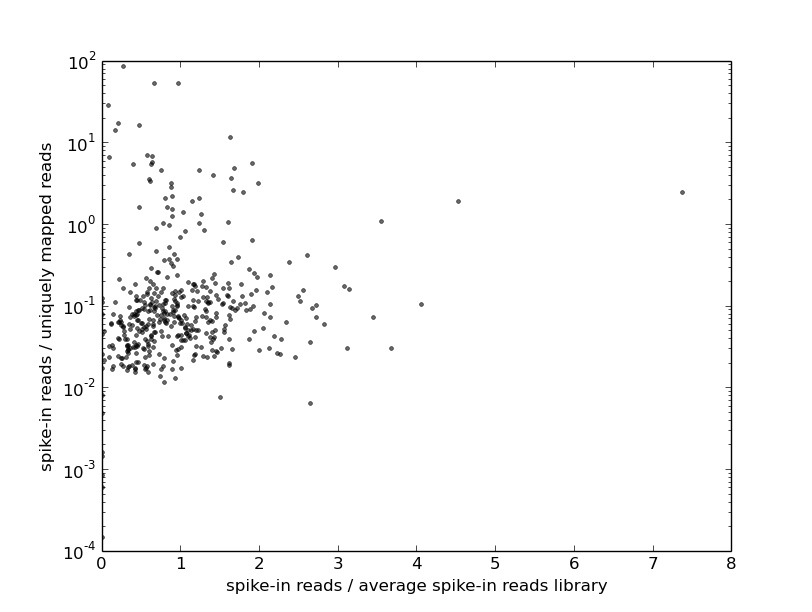
\includegraphics[width = 90mm]{figs/f1.jpg}    
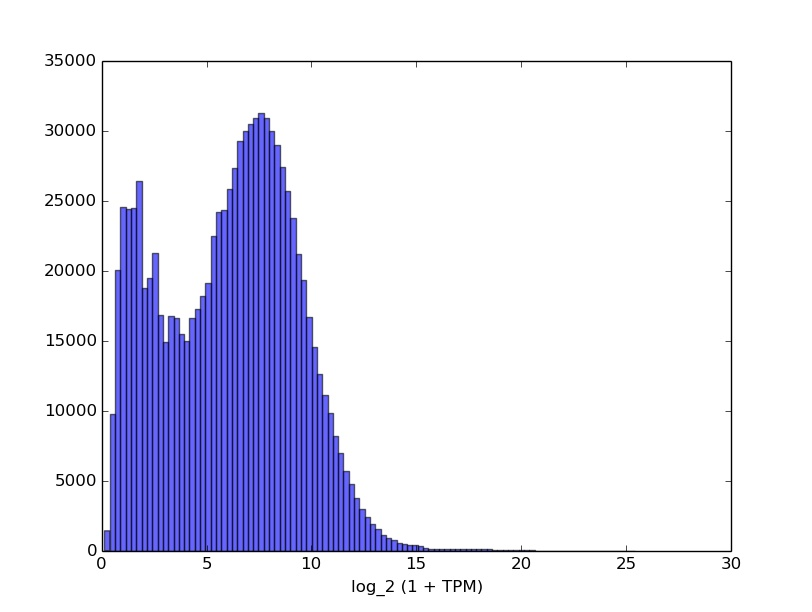
\includegraphics[width = 90mm]{figs/f2.jpg}    
\end{center}

From the first plot we observe that some cells have very low ratio
between spike-in reads and average spike-in reads in the library,
presumably due to low sequencing depth. Some other cells have large
ratio of spike-in reads and uniquely mapped reads, presumably due to
large amounts of degraded RNA. Finally, some cells have very low ratio
of spike-in reads and uniquely mapped reads, being large outliers. From
the second plot we observe a large amount of transcripts near the
detection limit, presumably due to noise.  When normalizing read counts to transcripts per million (TPM), SCTDA
assumes that read counts have been obtained by \href{http://www.ncbi.nlm.nih.gov/pubmed/22939981}{CEL-seq} or any other
single-cell RNA-seq method independent of gene lengths. 
We can filter out all those
cells using the method \texttt{SCTDA.Preprocess.save()}:

    % Make sure that atleast 4 lines are below the HR
    \needspace{4\baselineskip}

    
        \vspace{8pt}
        \makebox[0.1\linewidth]{\smaller\hfill\tt\color{nbframe-in-prompt}In\hspace{4pt}{[}4{]}:\hspace{4pt}}\\*
        \vspace{-2.1\baselineskip}
        \begin{ColorVerbatim}
            \vspace{-0.2\baselineskip}
            \begin{Verbatim}[commandchars=\\\{\}]
\PY{n}{p}\PY{o}{.}\PY{n}{save}\PY{p}{(}\PY{l+s}{\PYZsq{}}\PY{l+s}{table\PYZus{}tpm.tsv}\PY{l+s}{\PYZsq{}}\PY{p}{,} \PY{n}{filterXlow}\PY{o}{=}\PY{l+m+mf}{0.1}\PY{p}{,} \PY{n}{filterYlow}\PY{o}{=}\PY{l+m+mf}{0.01}\PY{p}{,} \PY{n}{filterYhigh}\PY{o}{=}\PY{l+m+mf}{0.8}\PY{p}{,} 
       \PY{n}{filterZlow}\PY{o}{=}\PY{l+m+mf}{4.0}\PY{p}{)}
\end{Verbatim}

            
                \vspace{-0.2\baselineskip}
            
        \end{ColorVerbatim}
    

    

        % If the first block is an image, minipage the image.  Else
        % request a certain amount of space for the input text.
        \needspace{4\baselineskip}
        
        

            % Add document contents.
            
                \makebox[0.1\linewidth]{\smaller\hfill\tt\color{nbframe-out-prompt}Out\hspace{4pt}{[}4{]}:\hspace{4pt}}\\*
                \vspace{-1.9\baselineskip}\begin{InvisibleVerbatim}
\begin{alltt}(373,
 \{'D2\_TM009.txt': 2,
  'D2\_TM010.txt': 5,
  'D3\_TM011.txt': 6,
  'D3\_TM012.txt': 4,
  'D4\_TM013.txt': 15,
  'D4\_TM015.txt': 6,
  'D5\_TM016.txt': 4,
  'D5\_TM019.txt': 6,
  'D6\_TM017.txt': 7,
  'D6\_TM018.txt': 11,
  'D6pos\_TM014.txt': 1\})\end{alltt}

            \end{InvisibleVerbatim}
            
        
    
Parameters \texttt{filterXlow} and \texttt{filterXhigh} set respectively lower and upper
bounds in the ratio between spike-in reads and the average number of
spike-in reads in the library. Parameters \texttt{filterYlow} and \texttt{filterYhigh} set
respectively lower and upper bounds in the ratio between spike-in reads
and uniquely mapped reads. Parameters \texttt{filterZlow} and \texttt{filterZhigh} set
respectively lower and upper bounds on the number of read counts for
each gene and sample. Out of the 440 cells, 373 pass all the above
filters. The number of cells that have been filtered out in each file is
returned as a dictionary.

The above command also produces a tab separated file called
\texttt{table\_tpm.tsv}, where each row correspond to a cell passing all filters.
The first column contains a unique identifier of the cell, the second
column contains the sampling day, the third column contains the library
id and the remaining columns contain $\textrm{log}_2(1+\textrm{TPM})$ expression values for
each gene, after filtering out reads according to \texttt{filterZlow} and
\texttt{filterZhigh} parameters. This table can be used by dedicated software,
such as \href{http://danifold.net/mapper/}{Mapper} or \href{http://www.ayasdi.com/}{Ayasdi}, to build a topological representation, that
can be then analysed using SCTDA.

\subsection{Parsing the topological graph}

Apart from the above tab separated table, SCTDA makes use of a
topological condensed representation of the table. This can be produced
using software such as \href{http://danifold.net/mapper/}{Mapper} or \href{http://www.ayasdi.com/}{Ayasdi}. The graph should be in GEXF
format, and should be accompanied by two JSON files with the same name
as the graph and extension \texttt{.json} and \texttt{.groups.json}, specifying
respectively the rows of the table that are associated to each node of
the graph and, optionally, groups of nodes to be considered for
subsequent analysis.

SCTDA provides a method to generate these files from an existing Ayasdi
Core session:

    % Make sure that atleast 4 lines are below the HR
    \needspace{4\baselineskip}

    
        \vspace{8pt}
        \makebox[0.1\linewidth]{\smaller\hfill\tt\color{nbframe-in-prompt}In\hspace{4pt}{[}5{]}:\hspace{4pt}}\\*
        \vspace{-2.1\baselineskip}
        \begin{ColorVerbatim}
            \vspace{-0.2\baselineskip}
            \begin{Verbatim}[commandchars=\\\{\}]
\PY{n}{SCTDA}\PY{o}{.}\PY{n}{ParseAyasdiGraph}\PY{p}{(}\PY{l+s}{\PYZdq{}}\PY{l+s}{analysis1}\PY{l+s}{\PYZdq{}}\PY{p}{,} \PY{l+s}{\PYZdq{}}\PY{l+s}{1436106543459}\PY{l+s}{\PYZdq{}}\PY{p}{,} 
                       \PY{l+s}{\PYZdq{}}\PY{l+s}{\PYZhy{}2007646151750978094}\PY{l+s}{\PYZdq{}}\PY{p}{,} \PY{l+s}{\PYZdq{}}\PY{l+s}{username}\PY{l+s}{\PYZdq{}}\PY{p}{,} \PY{l+s}{\PYZdq{}}\PY{l+s}{password}\PY{l+s}{\PYZdq{}}\PY{p}{)}\PY{p}{;}
\end{Verbatim}

            
                \vspace{-0.2\baselineskip}
            
        \end{ColorVerbatim}
    
This will produce the files \texttt{analysis1.gexf}, \texttt{analysis1.json} and
\texttt{analysis1.groups.json}. \texttt{``1436106543459''} and \texttt{``-2007646151750978094''}
are the identifiers of the Ayasdi Core session that we are importing
into SCTDA. They can be obtained from the Ayasdi Core session as
indicated in the following screenshot:
\begin{center}
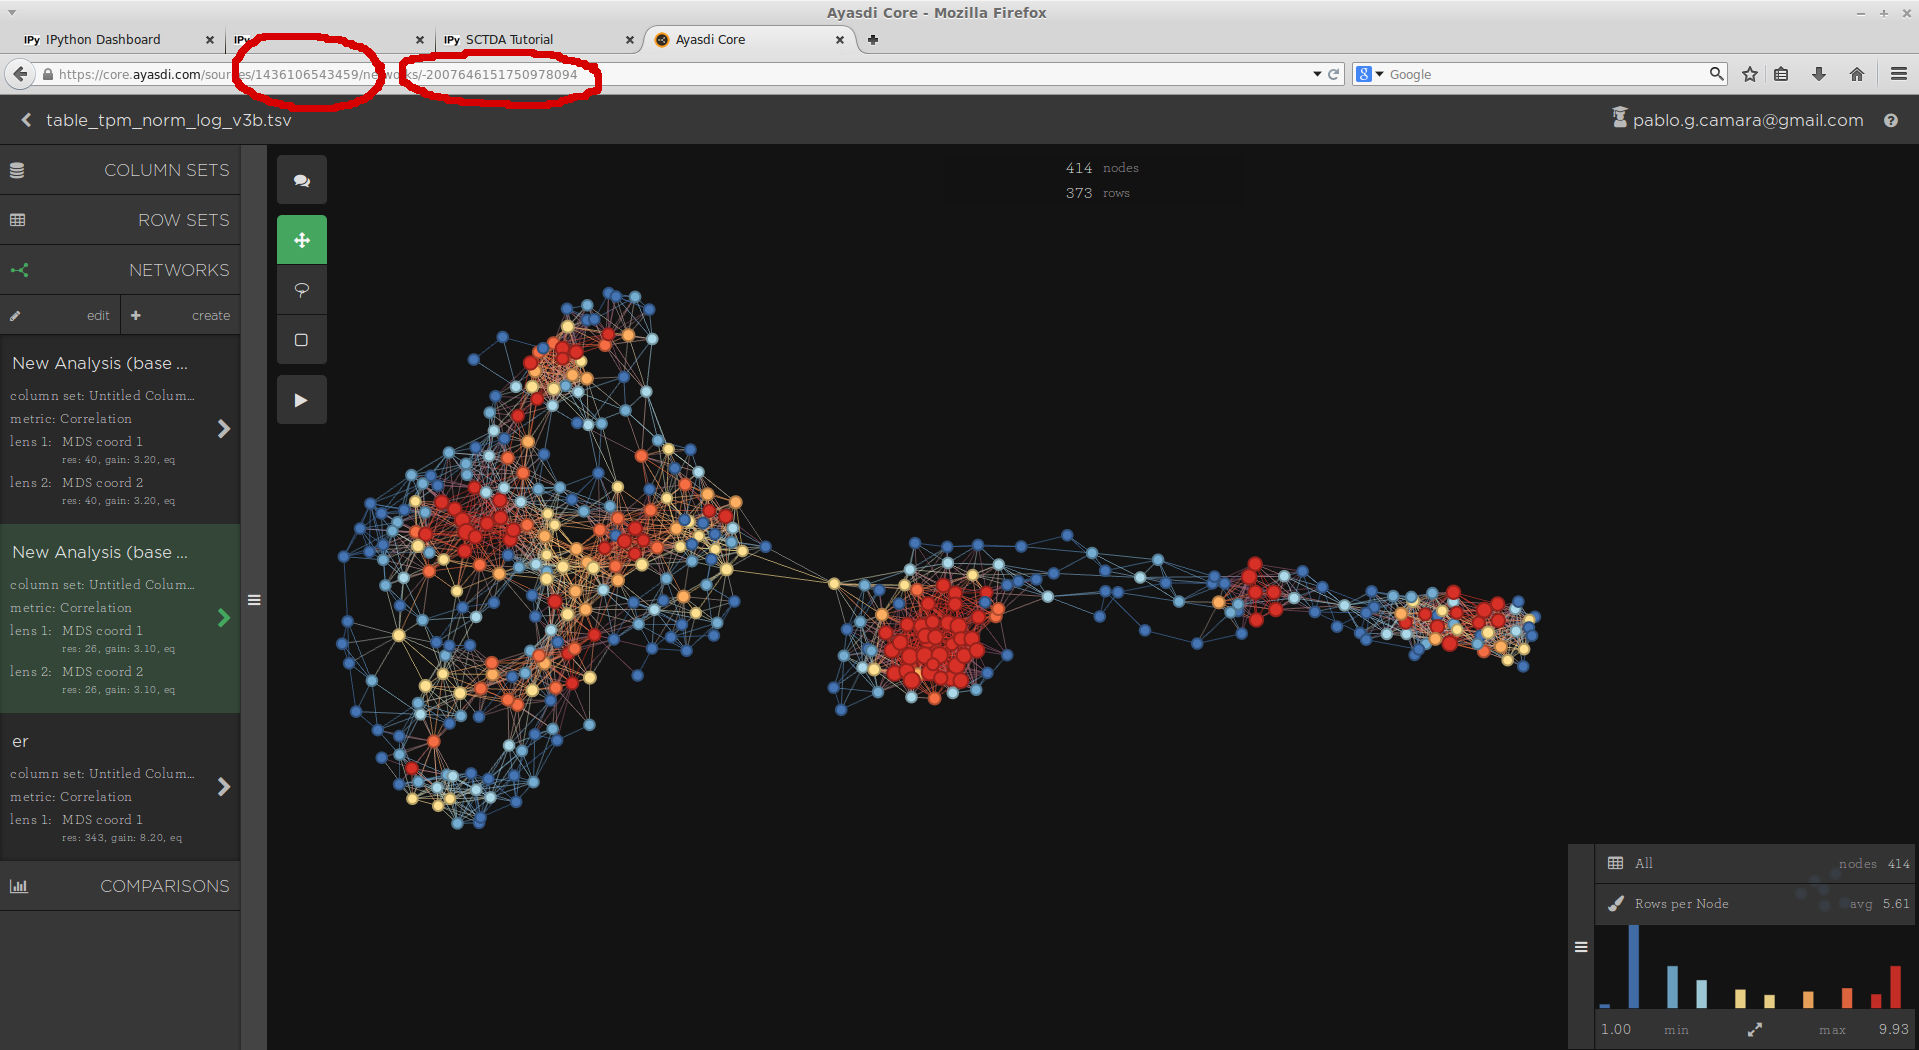
\includegraphics[width = 120mm]{figs/f3.jpg}    
\end{center}

\section{Analysis}

SCTDA provides two major classes for the analysis of single cell RNA-seq
expression data. These are \texttt{SCTDA.UnrootedGraph} and \texttt{SCTDA.RootedGraph},
respectively for non-longitudinal and longitudinal single cell RNA-seq
data. \texttt{SCTDA.RootedGraph} is an inherited class from \texttt{SCTDA.UnrootedGraph},
so all methods of \texttt{SCTDA.UnrootedGraph} are also included in
\texttt{SCTDA.RootedGraph}, in addition to some methods that are specific of
\texttt{SCTDA.RootedGraph}. In this tutorial we will make use of
\texttt{SCTDA.RootedGraph}, as we are dealing with longitudinal data. The class
is initialized with the data produced in the preliminary steps described
above:

    % Make sure that atleast 4 lines are below the HR
    \needspace{4\baselineskip}

    
        \vspace{8pt}
        \makebox[0.1\linewidth]{\smaller\hfill\tt\color{nbframe-in-prompt}In\hspace{4pt}{[}6{]}:\hspace{4pt}}\\*
        \vspace{-2.1\baselineskip}
        \begin{ColorVerbatim}
            \vspace{-0.2\baselineskip}
            \begin{Verbatim}[commandchars=\\\{\}]
\PY{n}{c} \PY{o}{=} \PY{n}{SCTDA}\PY{o}{.}\PY{n}{RootedGraph}\PY{p}{(}\PY{l+s}{\PYZdq{}}\PY{l+s}{analysis1}\PY{l+s}{\PYZdq{}}\PY{p}{,} \PY{l+s}{\PYZdq{}}\PY{l+s}{table\PYZus{}tpm.tsv}\PY{l+s}{\PYZdq{}}\PY{p}{)}\PY{p}{;}
\end{Verbatim}

            
                \vspace{-0.2\baselineskip}
            
        \end{ColorVerbatim}
    
The class includes several methods for the analysis and visualisation of
data. These are described in what follows.

\subsection{Exploring and visualizing the data}

We can display some general statistics using the method
\texttt{SCTDA.RootedGraph.show\_statistics()}:

    % Make sure that atleast 4 lines are below the HR
    \needspace{4\baselineskip}

    
        \vspace{8pt}
        \makebox[0.1\linewidth]{\smaller\hfill\tt\color{nbframe-in-prompt}In\hspace{4pt}{[}7{]}:\hspace{4pt}}\\*
        \vspace{-2.1\baselineskip}
        \begin{ColorVerbatim}
            \vspace{-0.2\baselineskip}
            \begin{Verbatim}[commandchars=\\\{\}]
\PY{n}{c}\PY{o}{.}\PY{n}{show\PYZus{}statistics}\PY{p}{(}\PY{p}{)}\PY{p}{;}
\end{Verbatim}

            
                \vspace{-0.2\baselineskip}
            
        \end{ColorVerbatim}

\begin{center}
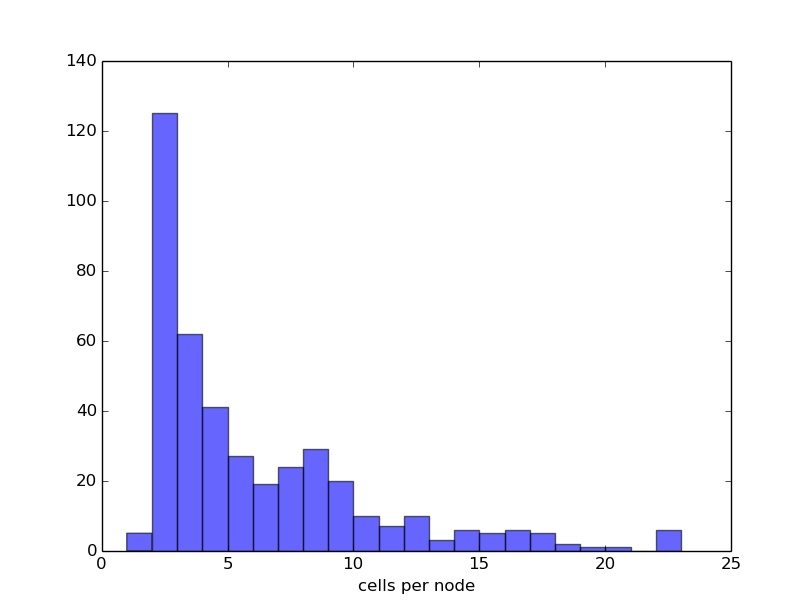
\includegraphics[width = 90mm]{figs/f4.jpg}    
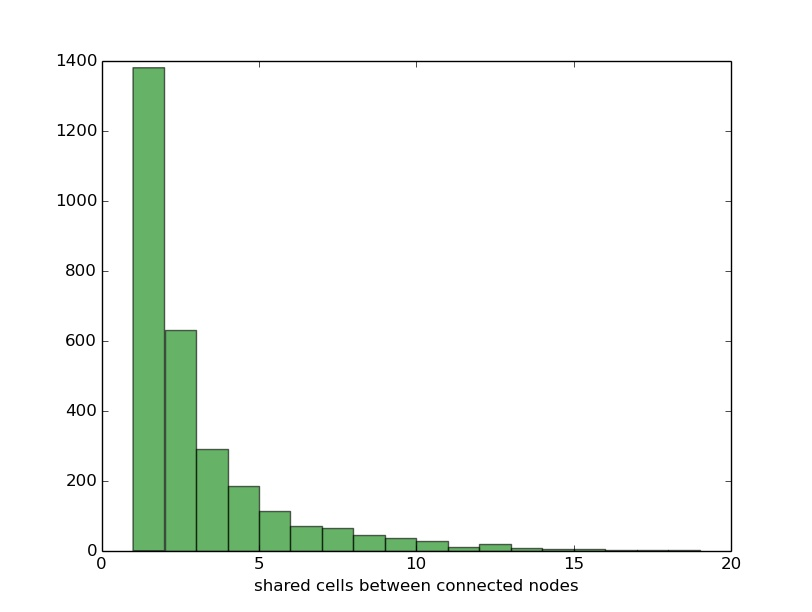
\includegraphics[width = 90mm]{figs/f5.jpg}    
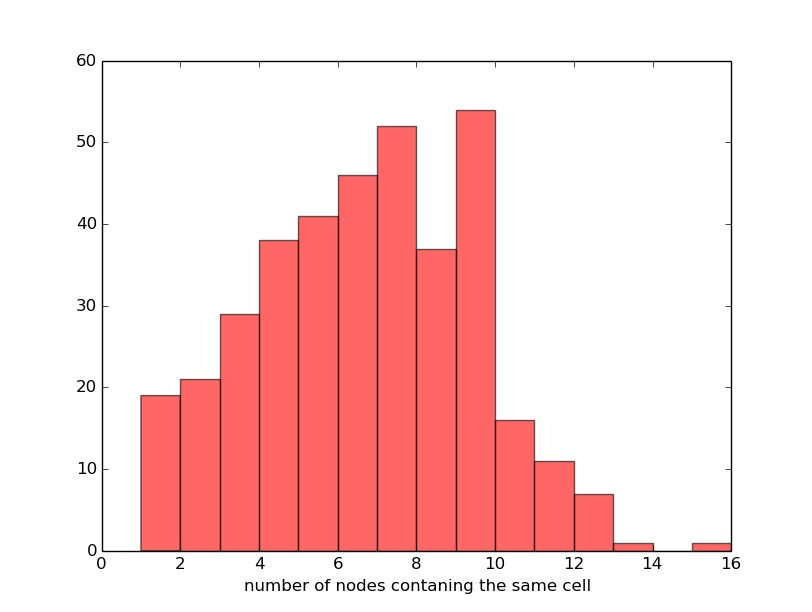
\includegraphics[width = 90mm]{figs/f6.jpg}    
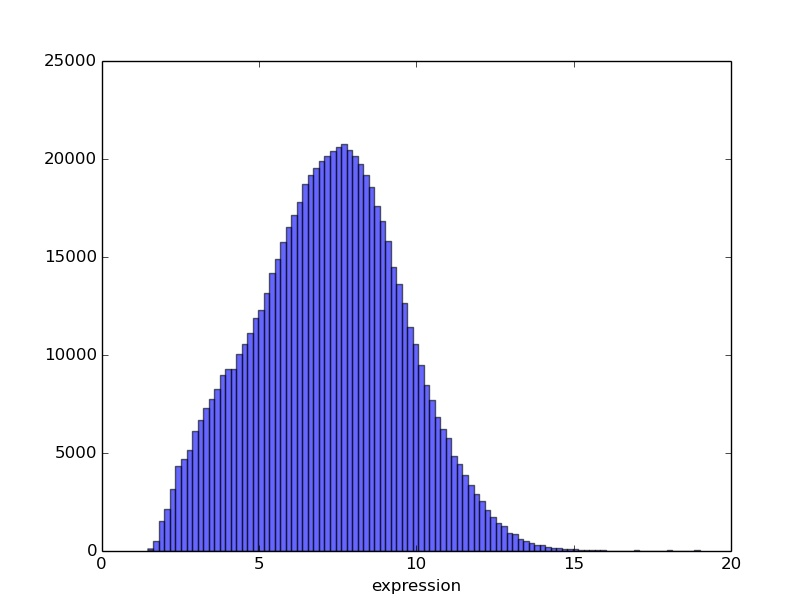
\includegraphics[width = 90mm]{figs/f7.jpg}    
\end{center}
    
The first plot displays the distribution of the number of cells per node in the
topological representation. The second plot presents the distribution of the
number of common cells between nodes that share an edge in the
topological representation. The third plot contains the distribution of the
number of nodes that contain the same cell. Last plot shows
the distribution of transcripts in $\textrm{log}_2(1+\textrm{TPM})$
scale, after filtering. Observe, in particular, that the filters that we have applied 
in the preliminary steps have removed the excess of transcripts near the detection limit.

We can use the method \texttt{SCTDA.RootedGraph.draw()} to display the topological
representation colored by the expression of a given gene:

    % Make sure that atleast 4 lines are below the HR
    \needspace{4\baselineskip}

    
        \vspace{8pt}
        \makebox[0.1\linewidth]{\smaller\hfill\tt\color{nbframe-in-prompt}In\hspace{4pt}{[}8{]}:\hspace{4pt}}\\*
        \vspace{-2.1\baselineskip}
        \begin{ColorVerbatim}
            \vspace{-0.2\baselineskip}
            \begin{Verbatim}[commandchars=\\\{\}]
\PY{n}{c}\PY{o}{.}\PY{n}{draw}\PY{p}{(}\PY{l+s}{\PYZsq{}}\PY{l+s}{Dnmt3b}\PY{l+s}{\PYZsq{}}\PY{p}{)}\PY{p}{;}
\end{Verbatim}

            
                \vspace{-0.2\baselineskip}
            
        \end{ColorVerbatim}

\begin{center}    
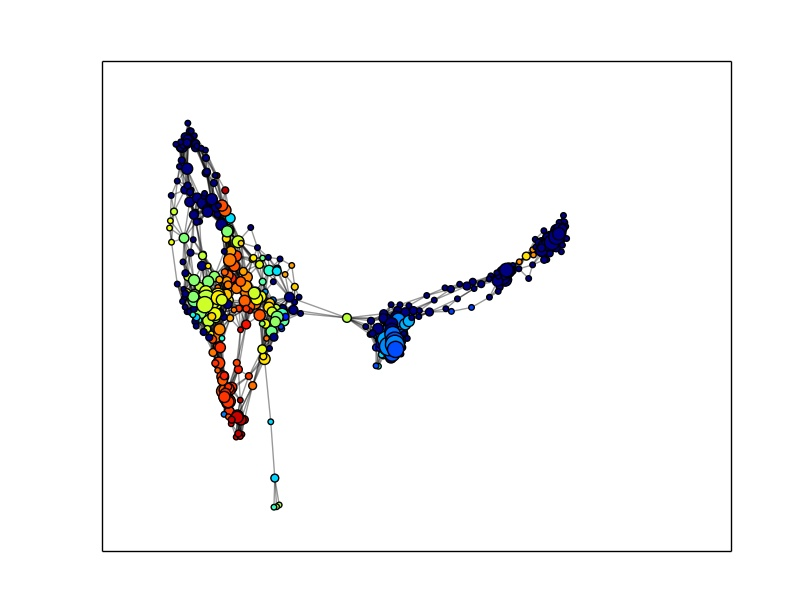
\includegraphics[width = 110mm]{figs/f8.jpg}    
\end{center}

Node sizes are proportional to the number of cells in the node.
The method \texttt{SCTDA.RootedGraph.draw()} also allows to map a gene or list of genes to
red, green and blue channels:

    % Make sure that atleast 4 lines are below the HR
    \needspace{4\baselineskip}

    
        \vspace{8pt}
        \makebox[0.1\linewidth]{\smaller\hfill\tt\color{nbframe-in-prompt}In\hspace{4pt}{[}9{]}:\hspace{4pt}}\\*
        \vspace{-2.1\baselineskip}
        \begin{ColorVerbatim}
            \vspace{-0.2\baselineskip}
            \begin{Verbatim}[commandchars=\\\{\}]
\PY{n}{c}\PY{o}{.}\PY{n}{draw}\PY{p}{(}\PY{p}{[}\PY{l+s}{\PYZsq{}}\PY{l+s}{Dnmt3b}\PY{l+s}{\PYZsq{}}\PY{p}{,}\PY{l+s}{\PYZsq{}}\PY{l+s}{Egfp}\PY{l+s}{\PYZsq{}}\PY{p}{,} \PY{l+s}{\PYZsq{}}\PY{l+s}{Foxa1}\PY{l+s}{\PYZsq{}}\PY{p}{]}\PY{p}{)}\PY{p}{;}
\end{Verbatim}

            
                \vspace{-0.2\baselineskip}
            
        \end{ColorVerbatim}

\begin{center}
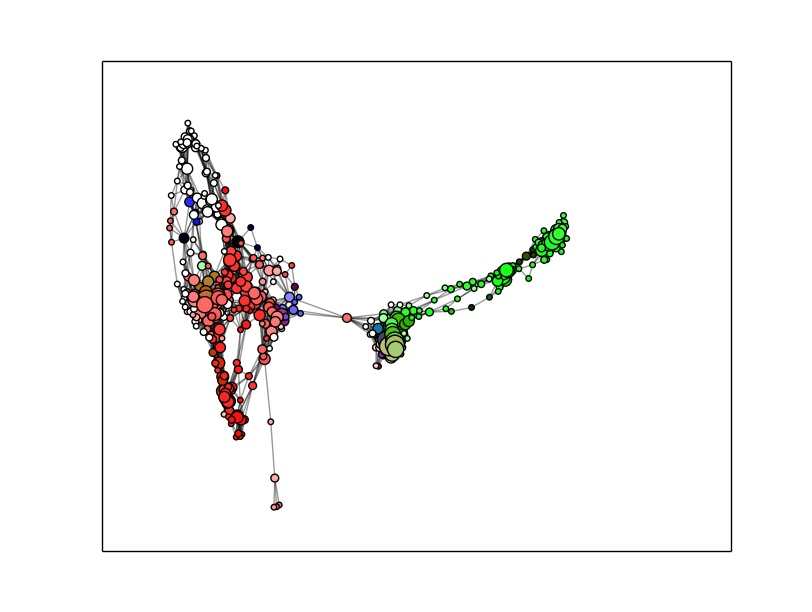
\includegraphics[width = 110mm]{figs/f9.jpg}    
\end{center}
    
With the option \texttt{table=True}, \texttt{SCTDA.RootedGraph.draw()} will also display some statistics (see
below for a more detailed description of each quantity):

    % Make sure that atleast 4 lines are below the HR
    \needspace{4\baselineskip}

    
        \vspace{8pt}
        \makebox[0.1\linewidth]{\smaller\hfill\tt\color{nbframe-in-prompt}In\hspace{4pt}{[}10{]}:\hspace{4pt}}\\*
        \vspace{-2.1\baselineskip}
        \begin{ColorVerbatim}
            \vspace{-0.2\baselineskip}
            \begin{Verbatim}[commandchars=\\\{\}]
\PY{n}{c}\PY{o}{.}\PY{n}{draw}\PY{p}{(}\PY{p}{[}\PY{l+s}{\PYZsq{}}\PY{l+s}{Dnmt3b}\PY{l+s}{\PYZsq{}}\PY{p}{,}\PY{l+s}{\PYZsq{}}\PY{l+s}{Egfp}\PY{l+s}{\PYZsq{}}\PY{p}{,} \PY{l+s}{\PYZsq{}}\PY{l+s}{Foxa1}\PY{l+s}{\PYZsq{}}\PY{p}{]}\PY{p}{,} \PY{n}{table}\PY{o}{=}\PY{n+nb+bp}{True}\PY{p}{)}\PY{p}{;}
\end{Verbatim}

                \vspace{-0.2\baselineskip}
            
        \end{ColorVerbatim}

\begin{center}
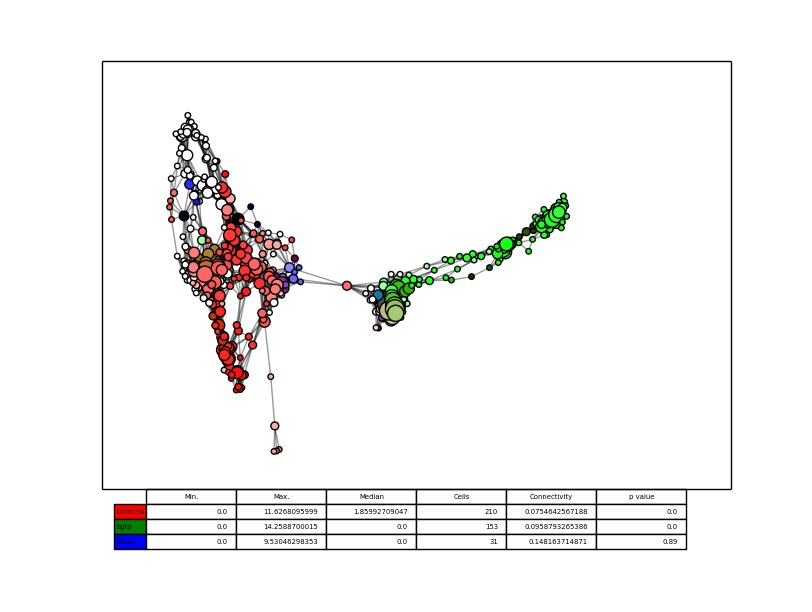
\includegraphics[width = 110mm]{figs/f10.jpg}    
\end{center}
    
\texttt{SCTDA.RootedGraph.draw()} is not limited to single genes, it can also map
lists of genes to a channel:

    % Make sure that atleast 4 lines are below the HR
    \needspace{4\baselineskip}

    
        \vspace{8pt}
        \makebox[0.1\linewidth]{\smaller\hfill\tt\color{nbframe-in-prompt}In\hspace{4pt}{[}11{]}:\hspace{4pt}}\\*
        \vspace{-2.1\baselineskip}
        \begin{ColorVerbatim}
            \vspace{-0.2\baselineskip}
            \begin{Verbatim}[commandchars=\\\{\}]
\PY{n}{c}\PY{o}{.}\PY{n}{draw}\PY{p}{(}\PY{p}{[}\PY{p}{[}\PY{l+s}{\PYZsq{}}\PY{l+s}{Dnmt3b}\PY{l+s}{\PYZsq{}}\PY{p}{,} \PY{l+s}{\PYZsq{}}\PY{l+s}{Dppa2}\PY{l+s}{\PYZsq{}}\PY{p}{,} \PY{l+s}{\PYZsq{}}\PY{l+s}{Dnmt3l}\PY{l+s}{\PYZsq{}}\PY{p}{]}\PY{p}{,}\PY{l+s}{\PYZsq{}}\PY{l+s}{Egfp}\PY{l+s}{\PYZsq{}}\PY{p}{,} \PY{l+s}{\PYZsq{}}\PY{l+s}{Foxa1}\PY{l+s}{\PYZsq{}}\PY{p}{]}\PY{p}{)}\PY{p}{;}
\end{Verbatim}

            
                \vspace{-0.2\baselineskip}
            
        \end{ColorVerbatim}

\begin{center}
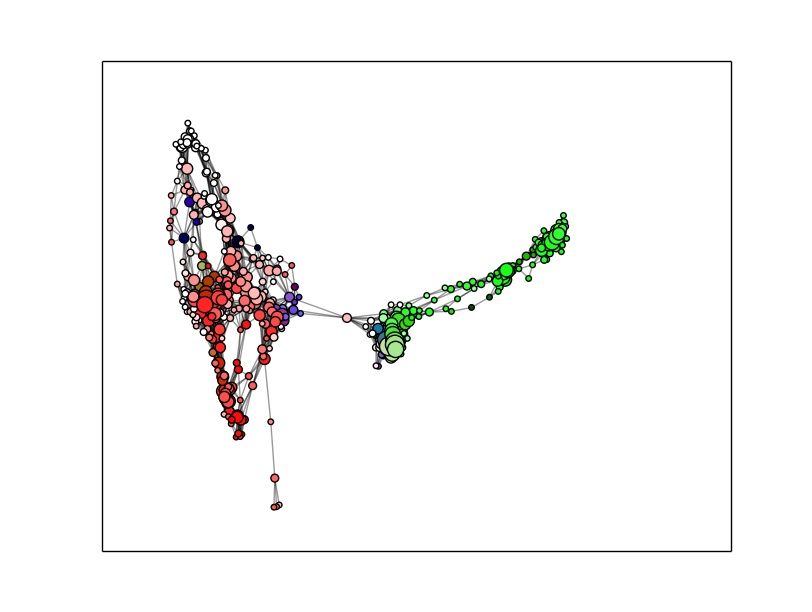
\includegraphics[width = 110mm]{figs/f11.jpg}    
\end{center}
    
\texttt{SCTDA.RootedGraph.draw()} also accepts some special keywords. The keyword
\texttt{`timepoint'} can be used to color according to the sampling time point:

    % Make sure that atleast 4 lines are below the HR
    \needspace{4\baselineskip}

    
        \vspace{8pt}
        \makebox[0.1\linewidth]{\smaller\hfill\tt\color{nbframe-in-prompt}In\hspace{4pt}{[}12{]}:\hspace{4pt}}\\*
        \vspace{-2.1\baselineskip}
        \begin{ColorVerbatim}
            \vspace{-0.2\baselineskip}
            \begin{Verbatim}[commandchars=\\\{\}]
\PY{n}{c}\PY{o}{.}\PY{n}{draw}\PY{p}{(}\PY{l+s}{\PYZsq{}}\PY{l+s}{timepoint}\PY{l+s}{\PYZsq{}}\PY{p}{)}\PY{p}{;}
\end{Verbatim}

            
                \vspace{-0.2\baselineskip}
            
        \end{ColorVerbatim}
    
\begin{center}
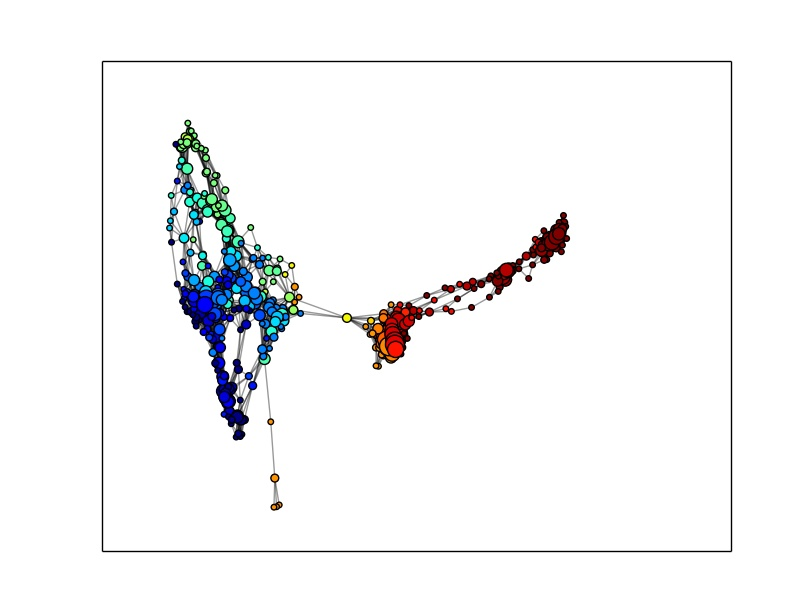
\includegraphics[width = 110mm]{figs/f12.jpg}    
\end{center}

A remarkable feature of the topological representation, based just on expression data, is that it correctly 
reproduces the differentiation time course, as observed in the above figure.

Similarly, the keyword \texttt{`timepoint\_'} can be used to plot the density of
cells of a given time point,

    % Make sure that atleast 4 lines are below the HR
    \needspace{4\baselineskip}

    
        \vspace{8pt}
        \makebox[0.1\linewidth]{\smaller\hfill\tt\color{nbframe-in-prompt}In\hspace{4pt}{[}13{]}:\hspace{4pt}}\\*
        \vspace{-2.1\baselineskip}
        \begin{ColorVerbatim}
            \vspace{-0.2\baselineskip}
            \begin{Verbatim}[commandchars=\\\{\}]
\PY{n}{c}\PY{o}{.}\PY{n}{draw}\PY{p}{(}\PY{l+s}{\PYZsq{}}\PY{l+s}{timepoint\PYZus{}5}\PY{l+s}{\PYZsq{}}\PY{p}{)}\PY{p}{;}
\end{Verbatim}

            
                \vspace{-0.2\baselineskip}
            
        \end{ColorVerbatim}

\begin{center}
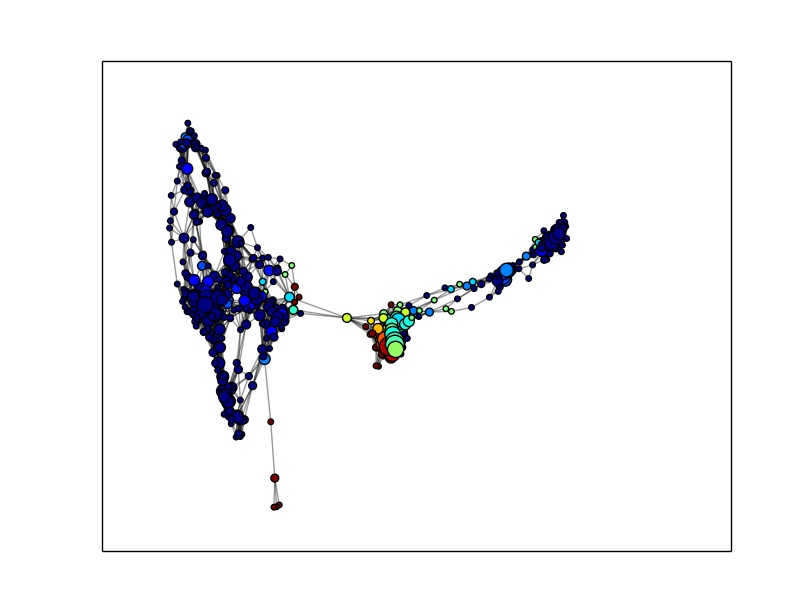
\includegraphics[width = 110mm]{figs/f13.jpg}    
\end{center}

SCTDA determines a root node in the topological representation by
maximizing the correlation between sampling time points and the graph
distance function. The root node corresponds to the less differentiated
state. We can color according to the distance to the root node using the
keyword \texttt{`\_dist\_root'},

    % Make sure that atleast 4 lines are below the HR
    \needspace{4\baselineskip}

    
        \vspace{8pt}
        \makebox[0.1\linewidth]{\smaller\hfill\tt\color{nbframe-in-prompt}In\hspace{4pt}{[}14{]}:\hspace{4pt}}\\*
        \vspace{-2.1\baselineskip}
        \begin{ColorVerbatim}
            \vspace{-0.2\baselineskip}
            \begin{Verbatim}[commandchars=\\\{\}]
\PY{n}{c}\PY{o}{.}\PY{n}{draw}\PY{p}{(}\PY{l+s}{\PYZsq{}}\PY{l+s}{\PYZus{}dist\PYZus{}root}\PY{l+s}{\PYZsq{}}\PY{p}{)}\PY{p}{;}
\end{Verbatim}

            
                \vspace{-0.2\baselineskip}
            
        \end{ColorVerbatim}

\begin{center}
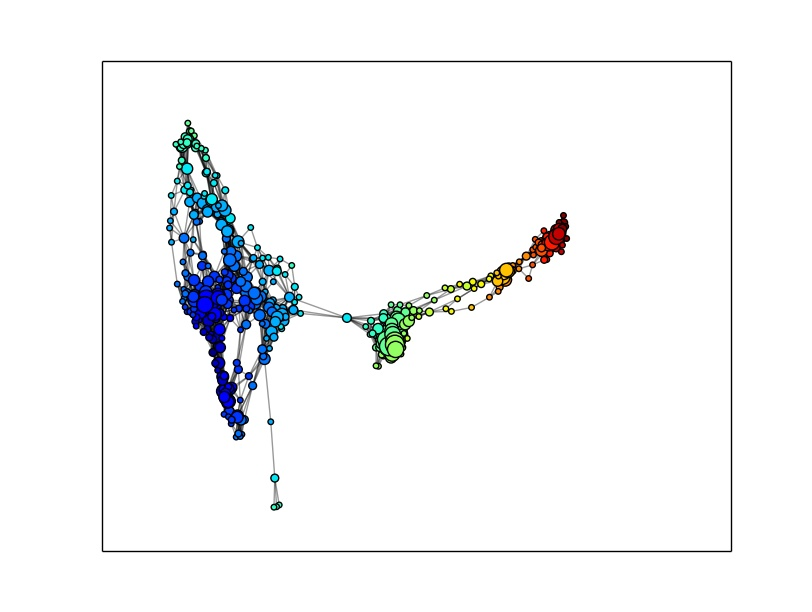
\includegraphics[width = 110mm]{figs/f14.jpg}    
\end{center}

Correlation between sampling time point and distance to root node can be
visualized using \texttt{SCTDA.RootedGraph.plot\_rootlane\_correlation()},

    % Make sure that atleast 4 lines are below the HR
    \needspace{4\baselineskip}

    
        \vspace{8pt}
        \makebox[0.1\linewidth]{\smaller\hfill\tt\color{nbframe-in-prompt}In\hspace{4pt}{[}15{]}:\hspace{4pt}}\\*
        \vspace{-2.1\baselineskip}
        \begin{ColorVerbatim}
            \vspace{-0.2\baselineskip}
            \begin{Verbatim}[commandchars=\\\{\}]
\PY{n}{c}\PY{o}{.}\PY{n}{plot\PYZus{}rootlane\PYZus{}correlation}\PY{p}{(}\PY{p}{)}
\end{Verbatim}

            
                \vspace{-0.2\baselineskip}
            
        \end{ColorVerbatim}
    

    

        % If the first block is an image, minipage the image.  Else
        % request a certain amount of space for the input text.
        \needspace{4\baselineskip}
        
        

            % Add document contents.
            
                \makebox[0.1\linewidth]{\smaller\hfill\tt\color{nbframe-out-prompt}Out\hspace{4pt}{[}15{]}:\hspace{4pt}}\\*
                \vspace{-1.9\baselineskip}\begin{InvisibleVerbatim}
\begin{alltt}(2.579181287149348,
 -3.5195814841484552,
 0.89109027529004081,
 2.2097001444641111e-141,
 0.065190844804728809)\end{alltt}

            \end{InvisibleVerbatim}
            
\begin{center}
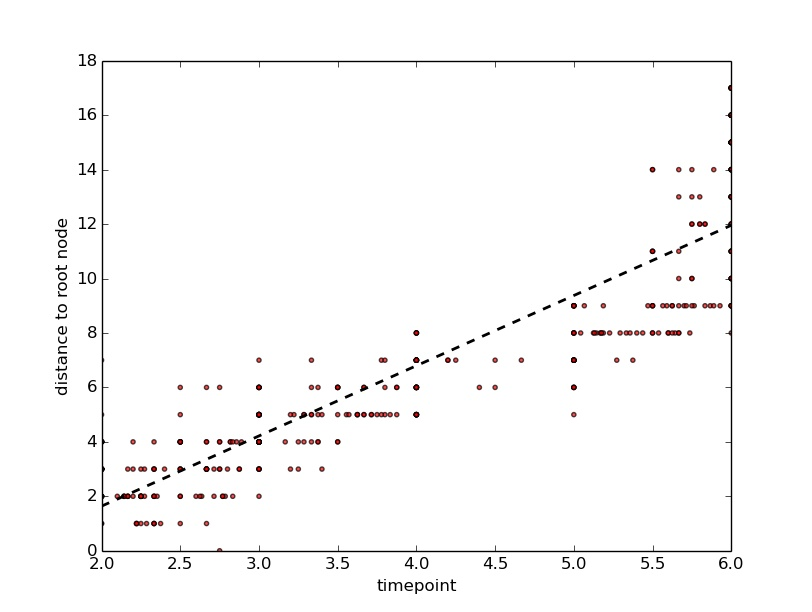
\includegraphics[width = 100mm]{figs/f15.jpg}    
\end{center}
        
    
\texttt{SCTDA.RootedGraph.plot\_rootlane\_correlation()} returns the two
parameters of the linear fit, Pearson's $r$, $p$-value and the standard
error.

The method \texttt{SCTDA.RootedGraph.draw\_expr\_timeline()} can be used to draw
the expression of a gene or list of genes at different time points, as
inferred from the distance to root function,

    % Make sure that atleast 4 lines are below the HR
    \needspace{4\baselineskip}

    
        \vspace{8pt}
        \makebox[0.1\linewidth]{\smaller\hfill\tt\color{nbframe-in-prompt}In\hspace{4pt}{[}16{]}:\hspace{4pt}}\\*
        \vspace{-2.1\baselineskip}
        \begin{ColorVerbatim}
            \vspace{-0.2\baselineskip}
            \begin{Verbatim}[commandchars=\\\{\}]
\PY{n}{c}\PY{o}{.}\PY{n}{draw\PYZus{}expr\PYZus{}timeline}\PY{p}{(}\PY{l+s}{\PYZsq{}}\PY{l+s}{Dnmt3b}\PY{l+s}{\PYZsq{}}\PY{p}{)}\PY{p}{;}
\end{Verbatim}

            
                \vspace{-0.2\baselineskip}
            
        \end{ColorVerbatim}
    
\begin{center}
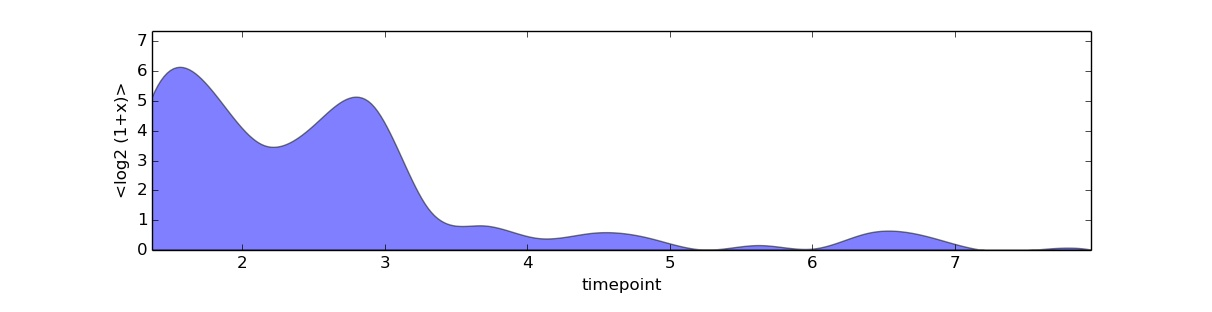
\includegraphics[width = 140mm]{figs/f16.jpg}    
\end{center}


    % Make sure that atleast 4 lines are below the HR
    \needspace{4\baselineskip}

    
        \vspace{8pt}
        \makebox[0.1\linewidth]{\smaller\hfill\tt\color{nbframe-in-prompt}In\hspace{4pt}{[}17{]}:\hspace{4pt}}\\*
        \vspace{-2.1\baselineskip}
        \begin{ColorVerbatim}
            \vspace{-0.2\baselineskip}
            \begin{Verbatim}[commandchars=\\\{\}]
\PY{n}{c}\PY{o}{.}\PY{n}{draw\PYZus{}expr\PYZus{}timeline}\PY{p}{(}\PY{p}{[}\PY{l+s}{\PYZsq{}}\PY{l+s}{Dnmt3b}\PY{l+s}{\PYZsq{}}\PY{p}{,} \PY{l+s}{\PYZsq{}}\PY{l+s}{Dppa2}\PY{l+s}{\PYZsq{}}\PY{p}{,} \PY{l+s}{\PYZsq{}}\PY{l+s}{Dnmt3l}\PY{l+s}{\PYZsq{}}\PY{p}{,} \PY{l+s}{\PYZsq{}}\PY{l+s}{Dppa4}\PY{l+s}{\PYZsq{}}\PY{p}{]}\PY{p}{)}\PY{p}{;}
\end{Verbatim}

            
                \vspace{-0.2\baselineskip}
            
        \end{ColorVerbatim}

\begin{center}
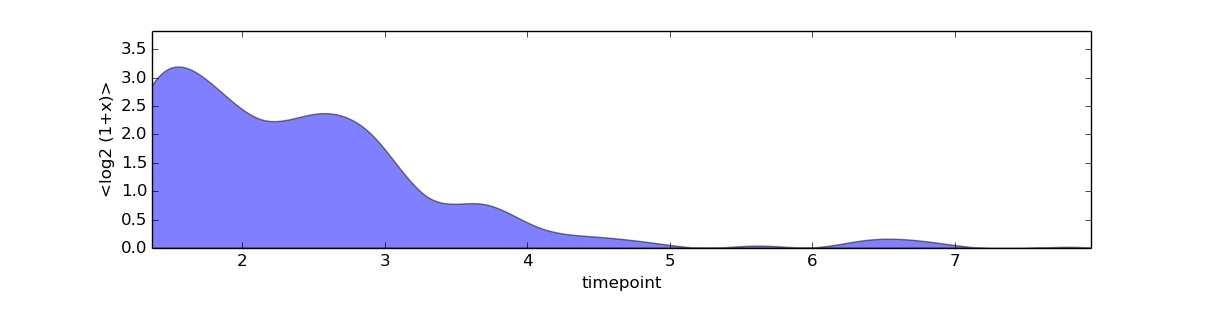
\includegraphics[width = 140mm]{figs/f17.jpg}    
\end{center}

Finally, we can display a skeleton of the differentiation tree
using \texttt{SCTDA.RootedGraph.draw\_skeleton()}, colored according to a gene or
list of genes, where each node in the skeleton corresponds to a set of
connected nodes at the same distance of the root node in the topological
condensed representation. Node sizes are proportional to the number of
cells in the node, whereas edge sizes are proportional to the number of
edges in the topological condensed representation connecting each pair
of group of nodes.

    % Make sure that atleast 4 lines are below the HR
    \needspace{4\baselineskip}

    
        \vspace{8pt}
        \makebox[0.1\linewidth]{\smaller\hfill\tt\color{nbframe-in-prompt}In\hspace{4pt}{[}18{]}:\hspace{4pt}}\\*
        \vspace{-2.1\baselineskip}
        \begin{ColorVerbatim}
            \vspace{-0.2\baselineskip}
            \begin{Verbatim}[commandchars=\\\{\}]
\PY{n}{c}\PY{o}{.}\PY{n}{draw\PYZus{}skeleton}\PY{p}{(}\PY{l+s}{\PYZsq{}}\PY{l+s}{Dnmt3b}\PY{l+s}{\PYZsq{}}\PY{p}{)}\PY{p}{;}
\end{Verbatim}

            
                \vspace{-0.2\baselineskip}
            
        \end{ColorVerbatim}

\begin{center}
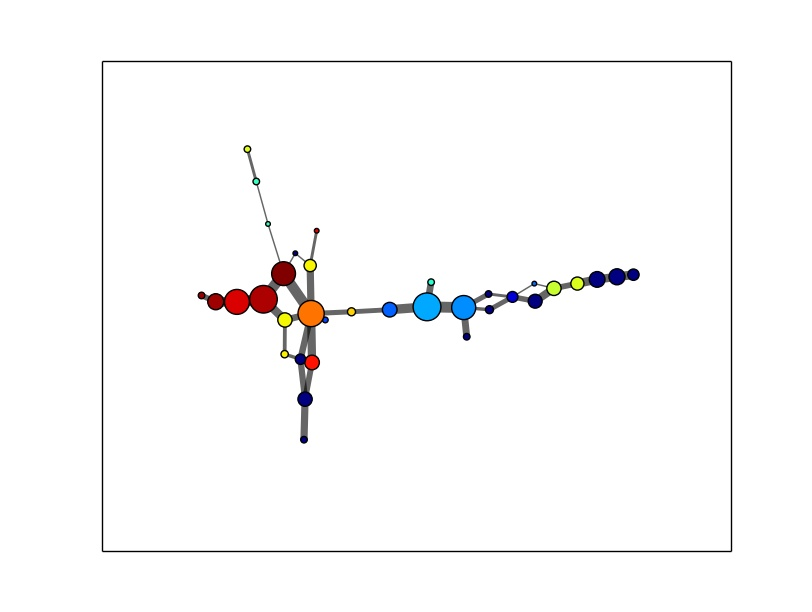
\includegraphics[width = 105mm]{figs/f18.jpg}    
\end{center}

    
\subsection{Connectivity, centroid and dispersion}

There are several quantities that can be associated to each gene and
that allow to identify genes that are specific of particular cell
sub-populations or time points. The first quantity that we may consider is
the connectivity of the expression of a gene in the topological
representation. This is defined as,
\begin{equation*}
S(g) = \frac{N-1}{N}\sum_{i,j} p_i(g) w_{ij} p_j(g)
\end{equation*}
where the sum runs over all nodes in the topological condensed
representation, $w$ is the adjacency matrix of the topological condensed
representation, $N$ the total number of nodes and $p_i(g)$ the average
expression of gene $g$ on node $i$, normalized as a probability, namely
\begin{equation*}
\sum_i p_i = 1
\end{equation*}
Connectivity allows to identify genes whose expression appears as highly
connected in the topological representation. The connectivity of a gene
can be computed using the method \texttt{SCTDA.RootedGraph.connectivity()},

    % Make sure that atleast 4 lines are below the HR
    \needspace{4\baselineskip}

    
        \vspace{8pt}
        \makebox[0.1\linewidth]{\smaller\hfill\tt\color{nbframe-in-prompt}In\hspace{4pt}{[}19{]}:\hspace{4pt}}\\*
        \vspace{-2.1\baselineskip}
        \begin{ColorVerbatim}
            \vspace{-0.2\baselineskip}
            \begin{Verbatim}[commandchars=\\\{\}]
\PY{n}{c}\PY{o}{.}\PY{n}{connectivity}\PY{p}{(}\PY{l+s}{\PYZsq{}}\PY{l+s}{Lhx3}\PY{l+s}{\PYZsq{}}\PY{p}{)}
\end{Verbatim}

            
                \vspace{-0.2\baselineskip}
            
        \end{ColorVerbatim}
    

    

        % If the first block is an image, minipage the image.  Else
        % request a certain amount of space for the input text.
        \needspace{4\baselineskip}
        
        

            % Add document contents.
            
                \makebox[0.1\linewidth]{\smaller\hfill\tt\color{nbframe-out-prompt}Out\hspace{4pt}{[}19{]}:\hspace{4pt}}\\*
                \vspace{-1.9\baselineskip}\begin{InvisibleVerbatim}
\begin{alltt}0.12959353154921011\end{alltt}

            \end{InvisibleVerbatim}
            
        
    
The statistical significance of a particular connectivity score can be
assessed by performing a permutation test, where cell labels are randomly
permuted. This is implemented in the method
\texttt{sctda.RottedGraph.connectivity\_pvalue()},

    % Make sure that atleast 4 lines are below the HR
    \needspace{4\baselineskip}

    
        \vspace{8pt}
        \makebox[0.1\linewidth]{\smaller\hfill\tt\color{nbframe-in-prompt}In\hspace{4pt}{[}20{]}:\hspace{4pt}}\\*
        \vspace{-2.1\baselineskip}
        \begin{ColorVerbatim}
            \vspace{-0.2\baselineskip}
            \begin{Verbatim}[commandchars=\\\{\}]
\PY{n}{c}\PY{o}{.}\PY{n}{connectivity\PYZus{}pvalue}\PY{p}{(}\PY{l+s}{\PYZsq{}}\PY{l+s}{Lhx3}\PY{l+s}{\PYZsq{}}\PY{p}{,} \PY{n}{n}\PY{o}{=}\PY{l+m+mi}{5000}\PY{p}{)}
\end{Verbatim}

            
                \vspace{-0.2\baselineskip}
            
        \end{ColorVerbatim}
    

    

        % If the first block is an image, minipage the image.  Else
        % request a certain amount of space for the input text.
        \needspace{4\baselineskip}
        
        

            % Add document contents.
            
                \makebox[0.1\linewidth]{\smaller\hfill\tt\color{nbframe-out-prompt}Out\hspace{4pt}{[}20{]}:\hspace{4pt}}\\*
                \vspace{-1.9\baselineskip}\begin{InvisibleVerbatim}
\begin{alltt}0.0\end{alltt}

            \end{InvisibleVerbatim}
            
        
    
where $n$ specifies the number of permutations. The idea is that genes
with a statistically significant connectivity, like the above example,
are biologically relevant at a particular stage or for a particular cell
sub-population,

    % Make sure that atleast 4 lines are below the HR
    \needspace{4\baselineskip}

    
        \vspace{8pt}
        \makebox[0.1\linewidth]{\smaller\hfill\tt\color{nbframe-in-prompt}In\hspace{4pt}{[}21{]}:\hspace{4pt}}\\*
        \vspace{-2.1\baselineskip}
        \begin{ColorVerbatim}
            \vspace{-0.2\baselineskip}
            \begin{Verbatim}[commandchars=\\\{\}]
\PY{n}{c}\PY{o}{.}\PY{n}{draw}\PY{p}{(}\PY{l+s}{\PYZsq{}}\PY{l+s}{Lhx3}\PY{l+s}{\PYZsq{}}\PY{p}{)}\PY{p}{;}
\end{Verbatim}

            
                \vspace{-0.2\baselineskip}
            
        \end{ColorVerbatim}

\begin{center}
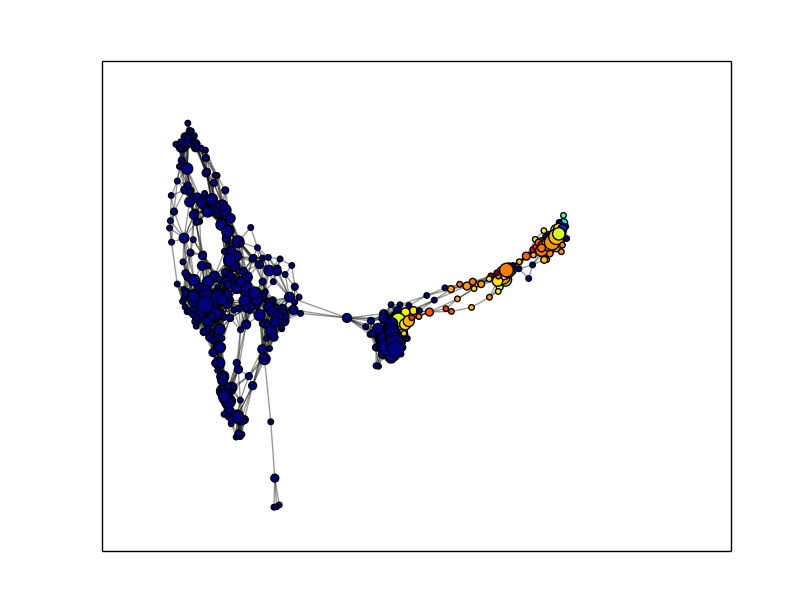
\includegraphics[width = 110mm]{figs/f19.jpg}    
\end{center}

On the contrary, genes with a non-significant connectivity in the
condensed topological representation are unspecific of any stage or cell
sub-population. For instance,

    % Make sure that atleast 4 lines are below the HR
    \needspace{4\baselineskip}

    
        \vspace{8pt}
        \makebox[0.1\linewidth]{\smaller\hfill\tt\color{nbframe-in-prompt}In\hspace{4pt}{[}22{]}:\hspace{4pt}}\\*
        \vspace{-2.1\baselineskip}
        \begin{ColorVerbatim}
            \vspace{-0.2\baselineskip}
            \begin{Verbatim}[commandchars=\\\{\}]
\PY{n}{c}\PY{o}{.}\PY{n}{connectivity\PYZus{}pvalue}\PY{p}{(}\PY{l+s}{\PYZsq{}}\PY{l+s}{St6gal1}\PY{l+s}{\PYZsq{}}\PY{p}{,} \PY{n}{n}\PY{o}{=}\PY{l+m+mi}{5000}\PY{p}{)}
\end{Verbatim}

            
                \vspace{-0.2\baselineskip}
            
        \end{ColorVerbatim}
    

    

        % If the first block is an image, minipage the image.  Else
        % request a certain amount of space for the input text.
        \needspace{4\baselineskip}
        
        

            % Add document contents.
            
                \makebox[0.1\linewidth]{\smaller\hfill\tt\color{nbframe-out-prompt}Out\hspace{4pt}{[}22{]}:\hspace{4pt}}\\*
                \vspace{-1.9\baselineskip}\begin{InvisibleVerbatim}
\begin{alltt}0.99880000000000002\end{alltt}

            \end{InvisibleVerbatim}
            
        
    


    % Make sure that atleast 4 lines are below the HR
    \needspace{4\baselineskip}

    
        \vspace{8pt}
        \makebox[0.1\linewidth]{\smaller\hfill\tt\color{nbframe-in-prompt}In\hspace{4pt}{[}23{]}:\hspace{4pt}}\\*
        \vspace{-2.1\baselineskip}
        \begin{ColorVerbatim}
            \vspace{-0.2\baselineskip}
            \begin{Verbatim}[commandchars=\\\{\}]
\PY{n}{c}\PY{o}{.}\PY{n}{draw}\PY{p}{(}\PY{l+s}{\PYZsq{}}\PY{l+s}{St6gal1}\PY{l+s}{\PYZsq{}}\PY{p}{)}\PY{p}{;}
\end{Verbatim}

            
                \vspace{-0.2\baselineskip}
            
        \end{ColorVerbatim}

\begin{center}
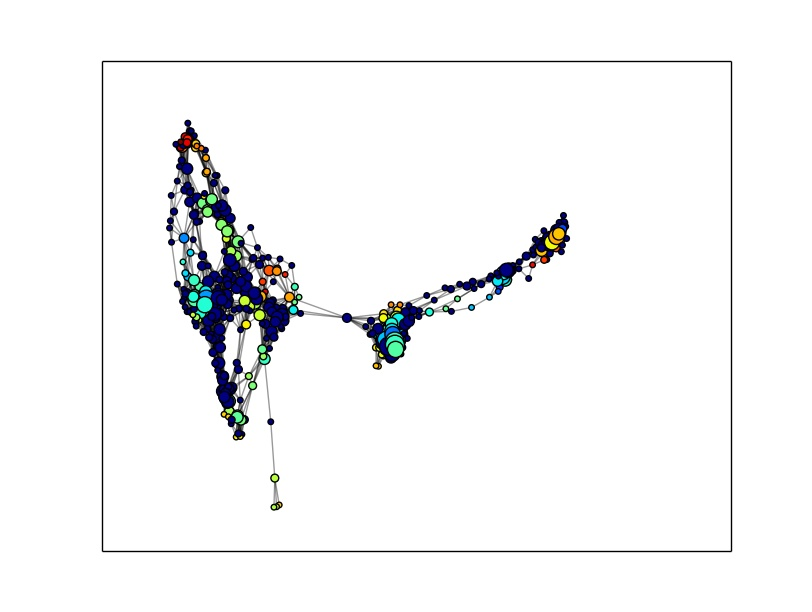
\includegraphics[width = 110mm]{figs/f20.jpg}    
\end{center}

Other interesting quantities are the centroid of a gene with respect to
the root node and its dispersion. These are respectively defined as

\begin{equation*}
C(g)=\sum_i d_i p_i(g)
\end{equation*}

\begin{equation*}
D(g) = \sqrt{\sum_i (d_i - C(g))^2p_i(g)}
\end{equation*}

where $d_i$ is the distance of node $i$ to the root node in the
topological representation.

The centroid and dispersion of a gene or list of genes can be computed
with the method \texttt{SCTDA.RootedGraph.centroid()},

    % Make sure that atleast 4 lines are below the HR
    \needspace{4\baselineskip}

    
        \vspace{8pt}
        \makebox[0.1\linewidth]{\smaller\hfill\tt\color{nbframe-in-prompt}In\hspace{4pt}{[}24{]}:\hspace{4pt}}\\*
        \vspace{-2.1\baselineskip}
        \begin{ColorVerbatim}
            \vspace{-0.2\baselineskip}
            \begin{Verbatim}[commandchars=\\\{\}]
\PY{n}{c}\PY{o}{.}\PY{n}{centroid}\PY{p}{(}\PY{l+s}{\PYZsq{}}\PY{l+s}{Lhx3}\PY{l+s}{\PYZsq{}}\PY{p}{)}
\end{Verbatim}

            
                \vspace{-0.2\baselineskip}
            
        \end{ColorVerbatim}
    

    

        % If the first block is an image, minipage the image.  Else
        % request a certain amount of space for the input text.
        \needspace{4\baselineskip}
        
        

            % Add document contents.
            
                \makebox[0.1\linewidth]{\smaller\hfill\tt\color{nbframe-out-prompt}Out\hspace{4pt}{[}24{]}:\hspace{4pt}}\\*
                \vspace{-1.9\baselineskip}\begin{InvisibleVerbatim}
\begin{alltt}[12.60030777275247, 2.5465951516563292]\end{alltt}

            \end{InvisibleVerbatim}
            
        
    
Other useful methods are \texttt{SCTDA.RootedGraph.expr()}, that returns the
number of cells on which expression of a gene or list of genes is
detected,

    % Make sure that atleast 4 lines are below the HR
    \needspace{4\baselineskip}

    
        \vspace{8pt}
        \makebox[0.1\linewidth]{\smaller\hfill\tt\color{nbframe-in-prompt}In\hspace{4pt}{[}25{]}:\hspace{4pt}}\\*
        \vspace{-2.1\baselineskip}
        \begin{ColorVerbatim}
            \vspace{-0.2\baselineskip}
            \begin{Verbatim}[commandchars=\\\{\}]
\PY{n}{c}\PY{o}{.}\PY{n}{expr}\PY{p}{(}\PY{l+s}{\PYZsq{}}\PY{l+s}{Lhx3}\PY{l+s}{\PYZsq{}}\PY{p}{)}
\end{Verbatim}

            
                \vspace{-0.2\baselineskip}
            
        \end{ColorVerbatim}
    

    

        % If the first block is an image, minipage the image.  Else
        % request a certain amount of space for the input text.
        \needspace{4\baselineskip}
        
        

            % Add document contents.
            
                \makebox[0.1\linewidth]{\smaller\hfill\tt\color{nbframe-out-prompt}Out\hspace{4pt}{[}25{]}:\hspace{4pt}}\\*
                \vspace{-1.9\baselineskip}\begin{InvisibleVerbatim}
\begin{alltt}93\end{alltt}

            \end{InvisibleVerbatim}
            
        
    
and \texttt{SCTDA.RootedGraph.delta()}, that returns the mean, minimum and
maximum expression values of a gene or list of genes,

    % Make sure that atleast 4 lines are below the HR
    \needspace{4\baselineskip}

    
        \vspace{8pt}
        \makebox[0.1\linewidth]{\smaller\hfill\tt\color{nbframe-in-prompt}In\hspace{4pt}{[}26{]}:\hspace{4pt}}\\*
        \vspace{-2.1\baselineskip}
        \begin{ColorVerbatim}
            \vspace{-0.2\baselineskip}
            \begin{Verbatim}[commandchars=\\\{\}]
\PY{n}{c}\PY{o}{.}\PY{n}{delta}\PY{p}{(}\PY{l+s}{\PYZsq{}}\PY{l+s}{Lhx3}\PY{l+s}{\PYZsq{}}\PY{p}{)}
\end{Verbatim}

            
                \vspace{-0.2\baselineskip}
            
        \end{ColorVerbatim}
    

    

        % If the first block is an image, minipage the image.  Else
        % request a certain amount of space for the input text.
        \needspace{4\baselineskip}
        
        

            % Add document contents.
            
                \makebox[0.1\linewidth]{\smaller\hfill\tt\color{nbframe-out-prompt}Out\hspace{4pt}{[}26{]}:\hspace{4pt}}\\*
                \vspace{-1.9\baselineskip}\begin{InvisibleVerbatim}
\begin{alltt}(1.5655427871802245, 0.0, 11.110091334383007)\end{alltt}

            \end{InvisibleVerbatim}
            
        
    
The methods \texttt{SCTDA.RootedGraph.expr()} and \texttt{SCTDA.RootedGraph.delta()} can
be restricted to specific groups of nodes. Groups of nodes are specified
in the file \texttt{name.groups.json} and stored in the dictionary
\texttt{SCTDA.RootedGraph.dicgroups}. For instance, in the example of this
tutorial we have defined three groups of nodes in the file
\texttt{analysis1.groups.json}. These can be accessed through

    % Make sure that atleast 4 lines are below the HR
    \needspace{4\baselineskip}

    
        \vspace{8pt}
        \makebox[0.1\linewidth]{\smaller\hfill\tt\color{nbframe-in-prompt}In\hspace{4pt}{[}27{]}:\hspace{4pt}}\\*
        \vspace{-2.1\baselineskip}
        \begin{ColorVerbatim}
            \vspace{-0.2\baselineskip}
            \begin{Verbatim}[commandchars=\\\{\}]
\PY{n}{c}\PY{o}{.}\PY{n}{dicgroups}\PY{o}{.}\PY{n}{keys}\PY{p}{(}\PY{p}{)}
\end{Verbatim}

            
                \vspace{-0.2\baselineskip}
            
        \end{ColorVerbatim}
    

    

        % If the first block is an image, minipage the image.  Else
        % request a certain amount of space for the input text.
        \needspace{4\baselineskip}
        
        

            % Add document contents.
            
                \makebox[0.1\linewidth]{\smaller\hfill\tt\color{nbframe-out-prompt}Out\hspace{4pt}{[}27{]}:\hspace{4pt}}\\*
                \vspace{-1.9\baselineskip}\begin{InvisibleVerbatim}
\begin{alltt}[u'Group\_3', u'Group\_2', u'Group\_1']\end{alltt}

            \end{InvisibleVerbatim}
            
        
    
We can restrict the commands \texttt{SCTDA.RootedGraph.expr()} and
\texttt{SCTDA.RootedGraph.delta()} to any of these groups by using the argument
\texttt{group=}. For instance,

    % Make sure that atleast 4 lines are below the HR
    \needspace{4\baselineskip}

    
        \vspace{8pt}
        \makebox[0.1\linewidth]{\smaller\hfill\tt\color{nbframe-in-prompt}In\hspace{4pt}{[}28{]}:\hspace{4pt}}\\*
        \vspace{-2.1\baselineskip}
        \begin{ColorVerbatim}
            \vspace{-0.2\baselineskip}
            \begin{Verbatim}[commandchars=\\\{\}]
\PY{n}{c}\PY{o}{.}\PY{n}{expr}\PY{p}{(}\PY{l+s}{\PYZsq{}}\PY{l+s}{Lhx3}\PY{l+s}{\PYZsq{}}\PY{p}{,} \PY{n}{group}\PY{o}{=}\PY{l+s}{\PYZsq{}}\PY{l+s}{Group\PYZus{}2}\PY{l+s}{\PYZsq{}}\PY{p}{)}
\end{Verbatim}

            
                \vspace{-0.2\baselineskip}
            
        \end{ColorVerbatim}
    

    

        % If the first block is an image, minipage the image.  Else
        % request a certain amount of space for the input text.
        \needspace{4\baselineskip}
        
        

            % Add document contents.
            
                \makebox[0.1\linewidth]{\smaller\hfill\tt\color{nbframe-out-prompt}Out\hspace{4pt}{[}28{]}:\hspace{4pt}}\\*
                \vspace{-1.9\baselineskip}\begin{InvisibleVerbatim}
\begin{alltt}22\end{alltt}

            \end{InvisibleVerbatim}
            
        
    


    % Make sure that atleast 4 lines are below the HR
    \needspace{4\baselineskip}

    
        \vspace{8pt}
        \makebox[0.1\linewidth]{\smaller\hfill\tt\color{nbframe-in-prompt}In\hspace{4pt}{[}29{]}:\hspace{4pt}}\\*
        \vspace{-2.1\baselineskip}
        \begin{ColorVerbatim}
            \vspace{-0.2\baselineskip}
            \begin{Verbatim}[commandchars=\\\{\}]
\PY{n}{c}\PY{o}{.}\PY{n}{delta}\PY{p}{(}\PY{l+s}{\PYZsq{}}\PY{l+s}{Lhx3}\PY{l+s}{\PYZsq{}}\PY{p}{,} \PY{n}{group}\PY{o}{=}\PY{l+s}{\PYZsq{}}\PY{l+s}{Group\PYZus{}2}\PY{l+s}{\PYZsq{}}\PY{p}{)}
\end{Verbatim}

            
                \vspace{-0.2\baselineskip}
            
        \end{ColorVerbatim}
    

    

        % If the first block is an image, minipage the image.  Else
        % request a certain amount of space for the input text.
        \needspace{4\baselineskip}
        
        

            % Add document contents.
            
                \makebox[0.1\linewidth]{\smaller\hfill\tt\color{nbframe-out-prompt}Out\hspace{4pt}{[}29{]}:\hspace{4pt}}\\*
                \vspace{-1.9\baselineskip}\begin{InvisibleVerbatim}
\begin{alltt}(1.8189051999362191, 0.0, 8.0067929633825727)\end{alltt}

            \end{InvisibleVerbatim}
            
        
    
The method \texttt{SCTDA.RootedGraph.save()} can be used to create a file called
\texttt{name.genes.tsv} containing a tab separated table with all the above
quantities for all genes in the dataset, including also Bejamini-Holchberg adjusted $p$-values for
the connectivity. This method allows to 
filter genes in that are expressed in more than \texttt{filtercells} cells, and
whose maximum expression value is above \texttt{filterexp} in
$\textrm{log}_2(1+\textrm{TPM})$ units. In addition, it allows to
annotate genes according to one or more lists of genes.

In the following example, we have downloaded from \href{http://www.ebi.ac.uk/QuickGO/}{EMBL-EBI QuickGO} two tables
listing the members of gene ontologies \emph{RNA splicing} and
\emph{Poly-(A) RNA binding}. We can parse the genes in those tables into
a dictionary that will be used by the command \texttt{SCTDA.RootedGraph.save()}
to annotate the genes:

    % Make sure that atleast 4 lines are below the HR
    \needspace{4\baselineskip}

    
        \vspace{8pt}
        \makebox[0.1\linewidth]{\smaller\hfill\tt\color{nbframe-in-prompt}In\hspace{4pt}{[}30{]}:\hspace{4pt}}\\*
        \vspace{-2.1\baselineskip}
        \begin{ColorVerbatim}
            \vspace{-0.2\baselineskip}
            \begin{Verbatim}[commandchars=\\\{\}]
\PY{n}{splic} \PY{o}{=} \PY{p}{[}\PY{p}{]}
\PY{n}{rna} \PY{o}{=} \PY{p}{[}\PY{p}{]}

\PY{n}{f} \PY{o}{=} \PY{n+nb}{open}\PY{p}{(}\PY{l+s}{\PYZsq{}}\PY{l+s}{GO0008380\PYZus{}RNA\PYZus{}spliciing.tsv}\PY{l+s}{\PYZsq{}}\PY{p}{,} \PY{l+s}{\PYZsq{}}\PY{l+s}{r}\PY{l+s}{\PYZsq{}}\PY{p}{)}
\PY{k}{for} \PY{n}{nb}\PY{p}{,} \PY{n}{line} \PY{o+ow}{in} \PY{n+nb}{enumerate}\PY{p}{(}\PY{n}{f}\PY{p}{)}\PY{p}{:}
    \PY{k}{if} \PY{n}{nb} \PY{o}{\PYZgt{}} \PY{l+m+mi}{0}\PY{p}{:}
        \PY{n}{sp} \PY{o}{=} \PY{n}{line}\PY{o}{.}\PY{n}{split}\PY{p}{(}\PY{l+s}{\PYZsq{}}\PY{l+s+se}{\PYZbs{}t}\PY{l+s}{\PYZsq{}}\PY{p}{)}
        \PY{n}{splic}\PY{o}{.}\PY{n}{append}\PY{p}{(}\PY{n}{sp}\PY{p}{[}\PY{l+m+mi}{2}\PY{p}{]}\PY{p}{)}
\PY{n}{f}\PY{o}{.}\PY{n}{close}\PY{p}{(}\PY{p}{)}
\PY{n}{splic} \PY{o}{=} \PY{n+nb}{list}\PY{p}{(}\PY{n+nb}{set}\PY{p}{(}\PY{n}{splic}\PY{p}{)}\PY{p}{)}

\PY{n}{f} \PY{o}{=} \PY{n+nb}{open}\PY{p}{(}\PY{l+s}{\PYZsq{}}\PY{l+s}{GO0044822\PYZus{}polyA\PYZus{}RNA\PYZus{}binding.tsv}\PY{l+s}{\PYZsq{}}\PY{p}{,} \PY{l+s}{\PYZsq{}}\PY{l+s}{r}\PY{l+s}{\PYZsq{}}\PY{p}{)}
\PY{k}{for} \PY{n}{nb}\PY{p}{,} \PY{n}{line} \PY{o+ow}{in} \PY{n+nb}{enumerate}\PY{p}{(}\PY{n}{f}\PY{p}{)}\PY{p}{:}
    \PY{k}{if} \PY{n}{nb} \PY{o}{\PYZgt{}} \PY{l+m+mi}{0}\PY{p}{:}
        \PY{n}{sp} \PY{o}{=} \PY{n}{line}\PY{o}{.}\PY{n}{split}\PY{p}{(}\PY{l+s}{\PYZsq{}}\PY{l+s+se}{\PYZbs{}t}\PY{l+s}{\PYZsq{}}\PY{p}{)}
        \PY{n}{rna}\PY{o}{.}\PY{n}{append}\PY{p}{(}\PY{n}{sp}\PY{p}{[}\PY{l+m+mi}{2}\PY{p}{]}\PY{p}{)}
\PY{n}{f}\PY{o}{.}\PY{n}{close}\PY{p}{(}\PY{p}{)}
\PY{n}{rna} \PY{o}{=} \PY{n+nb}{list}\PY{p}{(}\PY{n+nb}{set}\PY{p}{(}\PY{n}{rna}\PY{p}{)}\PY{p}{)}

\PY{n}{annotations} \PY{o}{=} \PY{p}{\PYZob{}}\PY{l+s}{\PYZsq{}}\PY{l+s}{Splicing}\PY{l+s}{\PYZsq{}}\PY{p}{:} \PY{n}{splic}\PY{p}{,} \PY{l+s}{\PYZsq{}}\PY{l+s}{RNA\PYZus{}binding}\PY{l+s}{\PYZsq{}}\PY{p}{:} \PY{n}{rna}\PY{p}{\PYZcb{}}
\end{Verbatim}

            
                \vspace{-0.2\baselineskip}
            
        \end{ColorVerbatim}
    
We use the method \texttt{SCTDA.RootedGraph.save()} to create the file
\texttt{analysis1.genes.tsv}, where we only consider genes that are expressed in
at least 3 cells and statistical significance is assessed using 500
permutations,

    % Make sure that atleast 4 lines are below the HR
    \needspace{4\baselineskip}

    
        \vspace{8pt}
        \makebox[0.1\linewidth]{\smaller\hfill\tt\color{nbframe-in-prompt}In\hspace{4pt}{[}31{]}:\hspace{4pt}}\\*
        \vspace{-2.1\baselineskip}
        \begin{ColorVerbatim}
            \vspace{-0.2\baselineskip}
            \begin{Verbatim}[commandchars=\\\{\}]
\PY{n}{c}\PY{o}{.}\PY{n}{save}\PY{p}{(}\PY{n}{n}\PY{o}{=}\PY{l+m+mi}{500}\PY{p}{,} \PY{n}{filtercells}\PY{o}{=}\PY{l+m+mi}{2}\PY{p}{,} \PY{n}{filterexp}\PY{o}{=}\PY{l+m+mf}{0.0}\PY{p}{,} \PY{n}{annotation}\PY{o}{=}\PY{n}{annotations}\PY{p}{)}\PY{p}{;}
\end{Verbatim}

            
                \vspace{-0.2\baselineskip}
            
        \end{ColorVerbatim}

\begin{center}
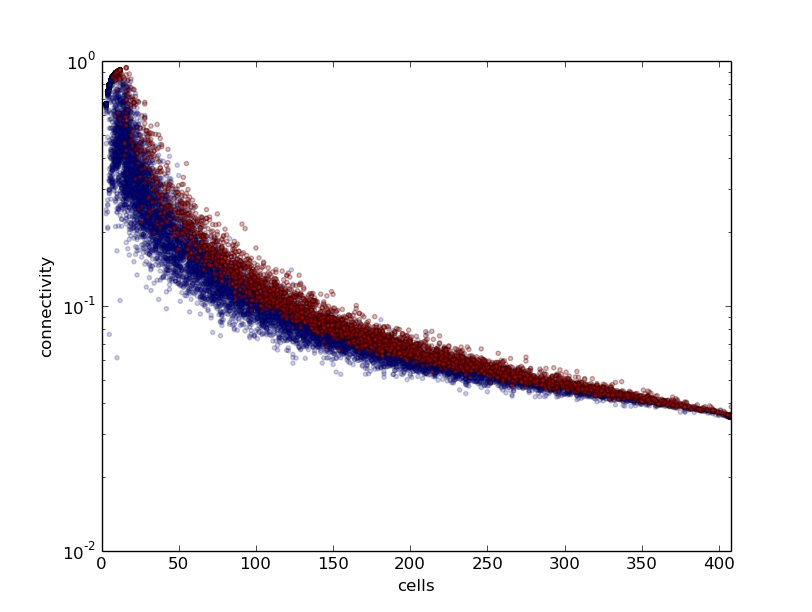
\includegraphics[width = 100mm]{figs/f21.jpg}    
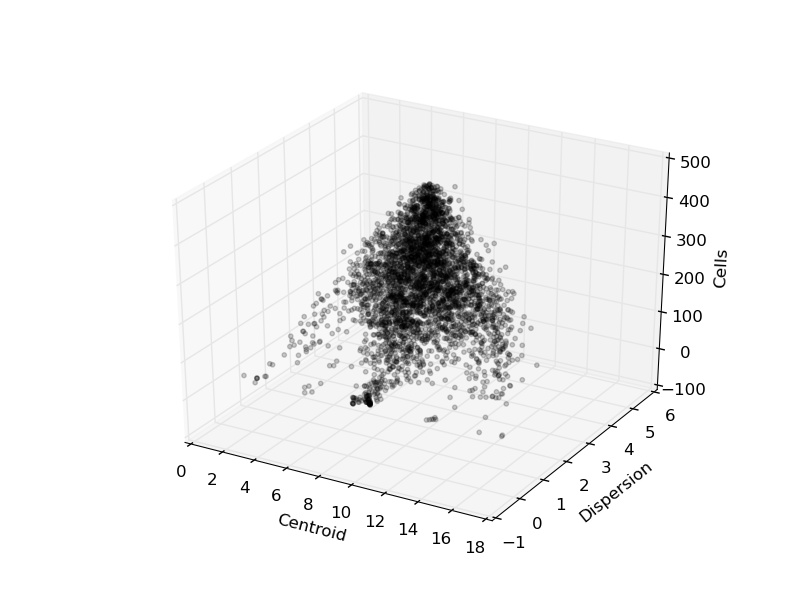
\includegraphics[width = 100mm]{figs/f22.jpg}    
\end{center}

    
\texttt{SCTDA.RootedGraph.save()} produces two plots. The first plot presents
connectivity against the number of cells with non-zero expression for
each gene. Genes with statistically significant connectivity, after
Benjamini-Holchberg adjustment for multiple testing, are displayed in
red. The second plot displays the number of cells with non-zero expression
against the centroid and dispersion, for genes with statistically
significant connectivity.

    % Make sure that atleast 4 lines are below the HR
    \needspace{4\baselineskip}

    
        \vspace{8pt}
        \makebox[0.1\linewidth]{\smaller\hfill\tt\color{nbframe-in-prompt}In\hspace{4pt}{[}32{]}:\hspace{4pt}}\\*
        \vspace{-2.1\baselineskip}
        \begin{ColorVerbatim}
            \vspace{-0.2\baselineskip}
            \begin{Verbatim}[commandchars=\\\{\}]
\PY{o}{!}head analysis1.genes.txt
\end{Verbatim}

            
                \vspace{-0.2\baselineskip}
            
        \end{ColorVerbatim}
    

    

        % If the first block is an image, minipage the image.  Else
        % request a certain amount of space for the input text.
        \needspace{4\baselineskip}
        
        

            % Add document contents.
            
                \begin{InvisibleVerbatim}
\begin{alltt}{\tiny      Gene     Cells     Mean    Min     Max  Connectivity p\_value BH p-value Centroid Dispersion RNA\_binding Splicing
0610005C13Rik   14      0.1986   0.0   7.69687   0.4918     0.348    0.4982    2.1365    0.3433        N         N
0610007N19Rik   49      0.3235   0.0   6.67145   0.2319     0.008    0.0349    7.7496    1.5264        N         N
0610007P14Rik   224     2.7506   0.0   7.98458   0.0597     0.0      0.0       6.9506    3.6452        N         N
0610009B22Rik   215     2.9831   0.0   9.45939   0.0620     0.016    0.0590    6.3790    3.5972        N         N
0610009D07Rik   266     4.1988   0.0   10.2019   0.0469     0.004    0.0202    7.3379    4.0085        N         N
0610009L18Rik   8       0.0907   0.0   5.09394   0.8762     0.284    0.4361    8.6537    0.4757        N         N
0610009O20Rik   137     1.0194   0.0   7.18446   0.0896     0.072    0.1735    7.2715    4.0472        N         N
0610010B08Rik   32      0.0802   0.0   4.10256   0.2968     0.15     0.2865    7.1221    2.0711        N         N
0610010F05Rik   192     2.6658   0.0   10.0240   0.0632     0.31     0.4629    7.7714    4.2535        N         N
}
\end{alltt}

            \end{InvisibleVerbatim}
            
        
    
\subsection{Adjacency and cell subpopulations}

A natural extension of the concept of connectivity to pairs of genes is
that of adjacency, defined as

\begin{equation*}
A(g,h) = \frac{N-1}{N}\sum_{i,j} p_i(g) w_{ij} p_j(h)
\end{equation*}

Adjacency takes high values when the expression of genes $g$ and $h$ are
adjacent to each other in the topological representation. Note that when
$g=h$, adjacency becomes connectivity.

The adjacency matrix of a list of genes can be computed in SCTDA using
the method,

    % Make sure that atleast 4 lines are below the HR
    \needspace{4\baselineskip}

    
        \vspace{8pt}
        \makebox[0.1\linewidth]{\smaller\hfill\tt\color{nbframe-in-prompt}In\hspace{4pt}{[}33{]}:\hspace{4pt}}\\*
        \vspace{-2.1\baselineskip}
        \begin{ColorVerbatim}
            \vspace{-0.2\baselineskip}
            \begin{Verbatim}[commandchars=\\\{\}]
\PY{n}{a} \PY{o}{=} \PY{n}{c}\PY{o}{.}\PY{n}{adjacency\PYZus{}matrix}\PY{p}{(}\PY{p}{[}\PY{l+s}{\PYZsq{}}\PY{l+s}{Dnmt3b}\PY{l+s}{\PYZsq{}}\PY{p}{,} \PY{l+s}{\PYZsq{}}\PY{l+s}{Dppa2}\PY{l+s}{\PYZsq{}}\PY{p}{,} \PY{l+s}{\PYZsq{}}\PY{l+s}{Dnmt3l}\PY{l+s}{\PYZsq{}}\PY{p}{,} \PY{l+s}{\PYZsq{}}\PY{l+s}{Dppa4}\PY{l+s}{\PYZsq{}}\PY{p}{,} \PY{l+s}{\PYZsq{}}\PY{l+s}{Lhx3}\PY{l+s}{\PYZsq{}}\PY{p}{]}\PY{p}{)}\PY{p}{;}
\PY{k}{print} \PY{n}{a}
\end{Verbatim}

            
                \vspace{-0.2\baselineskip}
            
        \end{ColorVerbatim}
    

    

        % If the first block is an image, minipage the image.  Else
        % request a certain amount of space for the input text.
        \needspace{4\baselineskip}
        
        

            % Add document contents.
            
                \begin{InvisibleVerbatim}
\begin{alltt}[[ 0.07546426  0.07197224  0.07238027  0.07201561  0.00710653]
 [ 0.07197224  0.09104796  0.08555381  0.07007939  0.        ]
 [ 0.07238027  0.08555381  0.11159461  0.07611521  0.        ]
 [ 0.07201561  0.07007939  0.07611521  0.08636352  0.0004148 ]
 [ 0.00710653  0.          0.          0.0004148   0.12959353]]
\end{alltt}

            \end{InvisibleVerbatim}
            
        
    
SCTDA makes use of adjacency and Jensen-Shannon distance to look for
potential cell sub-populations,

\begin{equation*}
J(g,h) = \left[\frac12\sum_i\left(p_i(g)\textrm{log }p_i(g)+p_i(h)\textrm{log }p_i(h)-(p_i(g)+p_i(h))\textrm{log }\frac{p_i(g)+p_i(h)}{2}\right)\right]^{\frac12}
\end{equation*}

Jensen-Shannon distance is implemented in SCTDA through the following method,

    % Make sure that atleast 4 lines are below the HR
    \needspace{4\baselineskip}

    
        \vspace{8pt}
        \makebox[0.1\linewidth]{\smaller\hfill\tt\color{nbframe-in-prompt}In\hspace{4pt}{[}34{]}:\hspace{4pt}}\\*
        \vspace{-2.1\baselineskip}
        \begin{ColorVerbatim}
            \vspace{-0.2\baselineskip}
            \begin{Verbatim}[commandchars=\\\{\}]
\PY{n}{b} \PY{o}{=} \PY{n}{c}\PY{o}{.}\PY{n}{JSD\PYZus{}matrix}\PY{p}{(}\PY{p}{[}\PY{l+s}{\PYZsq{}}\PY{l+s}{Dnmt3b}\PY{l+s}{\PYZsq{}}\PY{p}{,} \PY{l+s}{\PYZsq{}}\PY{l+s}{Dppa2}\PY{l+s}{\PYZsq{}}\PY{p}{,} \PY{l+s}{\PYZsq{}}\PY{l+s}{Dnmt3l}\PY{l+s}{\PYZsq{}}\PY{p}{,} \PY{l+s}{\PYZsq{}}\PY{l+s}{Dppa4}\PY{l+s}{\PYZsq{}}\PY{p}{,} \PY{l+s}{\PYZsq{}}\PY{l+s}{Lhx3}\PY{l+s}{\PYZsq{}}\PY{p}{]}\PY{p}{)}
\PY{k}{print} \PY{n}{b}
\end{Verbatim}

            
                \vspace{-0.2\baselineskip}
            
        \end{ColorVerbatim}
    

    

        % If the first block is an image, minipage the image.  Else
        % request a certain amount of space for the input text.
        \needspace{4\baselineskip}
        
        

            % Add document contents.
            
                \begin{InvisibleVerbatim}
\begin{alltt}[[ 0.          0.55105197  0.62788196  0.55417842  0.95451214]
 [ 0.55105197  0.          0.63299325  0.60159545  1.        ]
 [ 0.62788196  0.63299325  0.          0.66150927  1.        ]
 [ 0.55417842  0.60159545  0.66150927  0.          0.99758009]
 [ 0.95451214  1.          1.          0.99758009  0.        ]]
\end{alltt}

            \end{InvisibleVerbatim}
            
        
    
Adjacency and Jensen-Shannon distance are used by \texttt{SCTDA.RootedGraph.candidate\_subpopulations()} to look for potential cell sub-populations in a rather unsupervised way. We end this tutorial by illustrating the use of this method. The 3-dimensional plot produced by
\texttt{SCTDA.RootedGraph.save()} for our particular example showed three
``flares'' corresponding to three sets of genes with low dispersion and
statistically significant connectivity corresponding to centroids in
three different ranges. Let us consider the second group (corresponding
to progenitor motor neurons),

    % Make sure that atleast 4 lines are below the HR
    \needspace{4\baselineskip}

    
        \vspace{8pt}
        \makebox[0.1\linewidth]{\smaller\hfill\tt\color{nbframe-in-prompt}In\hspace{4pt}{[}35{]}:\hspace{4pt}}\\*
        \vspace{-2.1\baselineskip}
        \begin{ColorVerbatim}
            \vspace{-0.2\baselineskip}
            \begin{Verbatim}[commandchars=\\\{\}]
\PY{n}{group2} \PY{o}{=} \PY{p}{[}\PY{p}{]}
\PY{n}{f} \PY{o}{=} \PY{n+nb}{open}\PY{p}{(}\PY{l+s}{\PYZsq{}}\PY{l+s}{analysis1.genes.txt}\PY{l+s}{\PYZsq{}}\PY{p}{,} \PY{l+s}{\PYZsq{}}\PY{l+s}{r}\PY{l+s}{\PYZsq{}}\PY{p}{)}
\PY{k}{for} \PY{n}{n}\PY{p}{,} \PY{n}{line} \PY{o+ow}{in} \PY{n+nb}{enumerate}\PY{p}{(}\PY{n}{f}\PY{p}{)}\PY{p}{:}
    \PY{k}{if} \PY{n}{n}\PY{o}{\PYZgt{}}\PY{l+m+mi}{0}\PY{p}{:}
        \PY{n}{sp} \PY{o}{=} \PY{n}{line}\PY{p}{[}\PY{p}{:}\PY{o}{\PYZhy{}}\PY{l+m+mi}{1}\PY{p}{]}\PY{o}{.}\PY{n}{split}\PY{p}{(}\PY{l+s}{\PYZsq{}}\PY{l+s+se}{\PYZbs{}t}\PY{l+s}{\PYZsq{}}\PY{p}{)}
        \PY{k}{if} \PY{n+nb}{float}\PY{p}{(}\PY{n}{sp}\PY{p}{[}\PY{l+m+mi}{7}\PY{p}{]}\PY{p}{)} \PY{o}{\PYZlt{}}\PY{o}{=} \PY{l+m+mf}{0.05} \PY{o+ow}{and} \PY{l+m+mf}{7.5} \PY{o}{\PYZlt{}} \PY{n+nb}{float}\PY{p}{(}\PY{n}{sp}\PY{p}{[}\PY{l+m+mi}{8}\PY{p}{]}\PY{p}{)} \PY{o}{\PYZlt{}} \PY{l+m+mf}{8.8} 
                                          \PY{o+ow}{and} \PY{n+nb}{float}\PY{p}{(}\PY{n}{sp}\PY{p}{[}\PY{l+m+mi}{9}\PY{p}{]}\PY{p}{)} \PY{o}{\PYZlt{}} \PY{l+m+mf}{1.9}\PY{p}{:}
            \PY{n}{group2}\PY{o}{.}\PY{n}{append}\PY{p}{(}\PY{n}{sp}\PY{p}{[}\PY{l+m+mi}{0}\PY{p}{]}\PY{p}{)}
\PY{n}{f}\PY{o}{.}\PY{n}{close}\PY{p}{(}\PY{p}{)}
\end{Verbatim}

            
                \vspace{-0.2\baselineskip}
            
        \end{ColorVerbatim}
    


    % Make sure that atleast 4 lines are below the HR
    \needspace{4\baselineskip}

    
        \vspace{8pt}
        \makebox[0.1\linewidth]{\smaller\hfill\tt\color{nbframe-in-prompt}In\hspace{4pt}{[}36{]}:\hspace{4pt}}\\*
        \vspace{-2.1\baselineskip}
        \begin{ColorVerbatim}
            \vspace{-0.2\baselineskip}
            \begin{Verbatim}[commandchars=\\\{\}]
\PY{n}{c}\PY{o}{.}\PY{n}{draw}\PY{p}{(}\PY{p}{[}\PY{n}{group2}\PY{p}{]}\PY{p}{)}\PY{p}{;}
\end{Verbatim}

            
                \vspace{-0.2\baselineskip}
            
        \end{ColorVerbatim}

\begin{center}
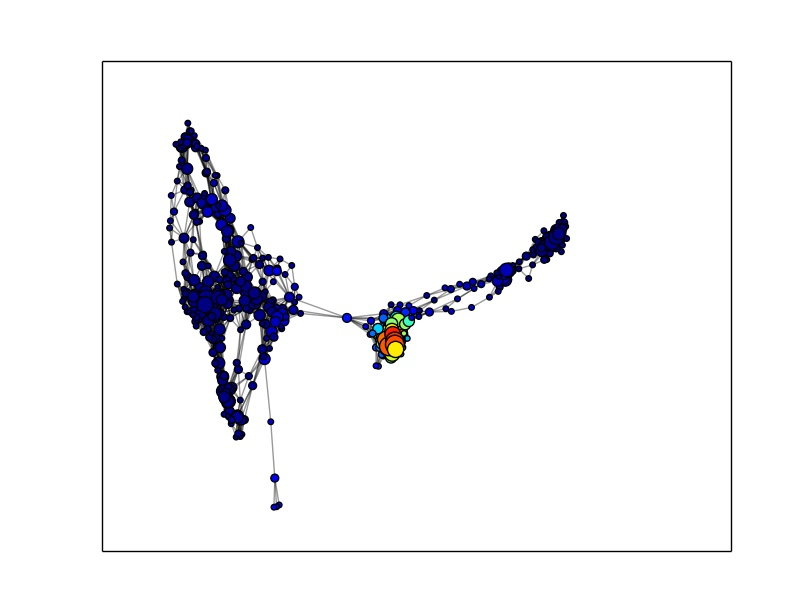
\includegraphics[width = 110mm]{figs/f23.jpg}    
\end{center}
    
A list of potential cell sub-populations based on these genes can be
produced using the method \texttt{SCTDA.RootedGraph.candidate\_supopoulations()},

    % Make sure that atleast 4 lines are below the HR
    \needspace{4\baselineskip}

    
        \vspace{8pt}
        \makebox[0.1\linewidth]{\smaller\hfill\tt\color{nbframe-in-prompt}In\hspace{4pt}{[}37{]}:\hspace{4pt}}\\*
        \vspace{-2.1\baselineskip}
        \begin{ColorVerbatim}
            \vspace{-0.2\baselineskip}
            \begin{Verbatim}[commandchars=\\\{\}]
\PY{n}{u} \PY{o}{=} \PY{n}{c}\PY{o}{.}\PY{n}{candidate\PYZus{}subpopulations}\PY{p}{(}\PY{n}{group2}\PY{p}{,} \PY{n}{thres}\PY{o}{=}\PY{l+m+mf}{0.05}\PY{p}{)}\PY{p}{;}
\end{Verbatim}

            
                \vspace{-0.2\baselineskip}
            
        \end{ColorVerbatim}

\begin{center}
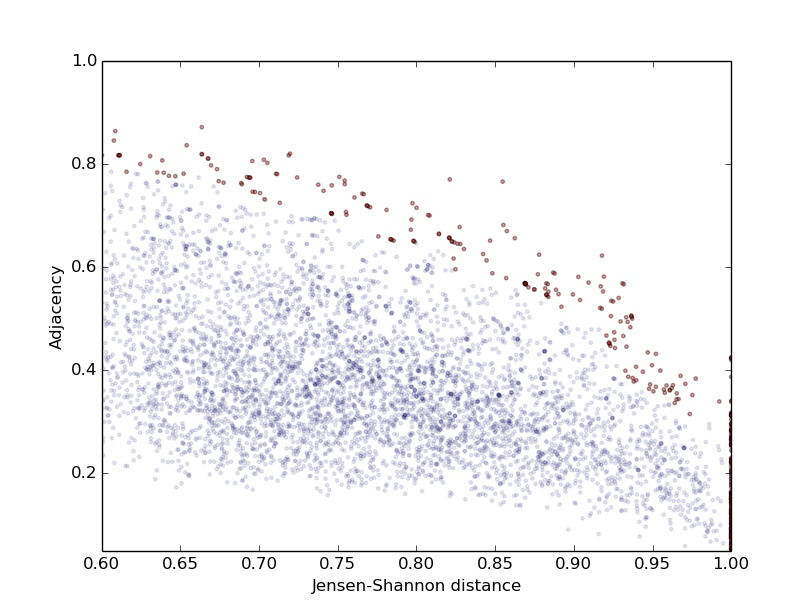
\includegraphics[width = 90mm]{figs/f24.jpg}    
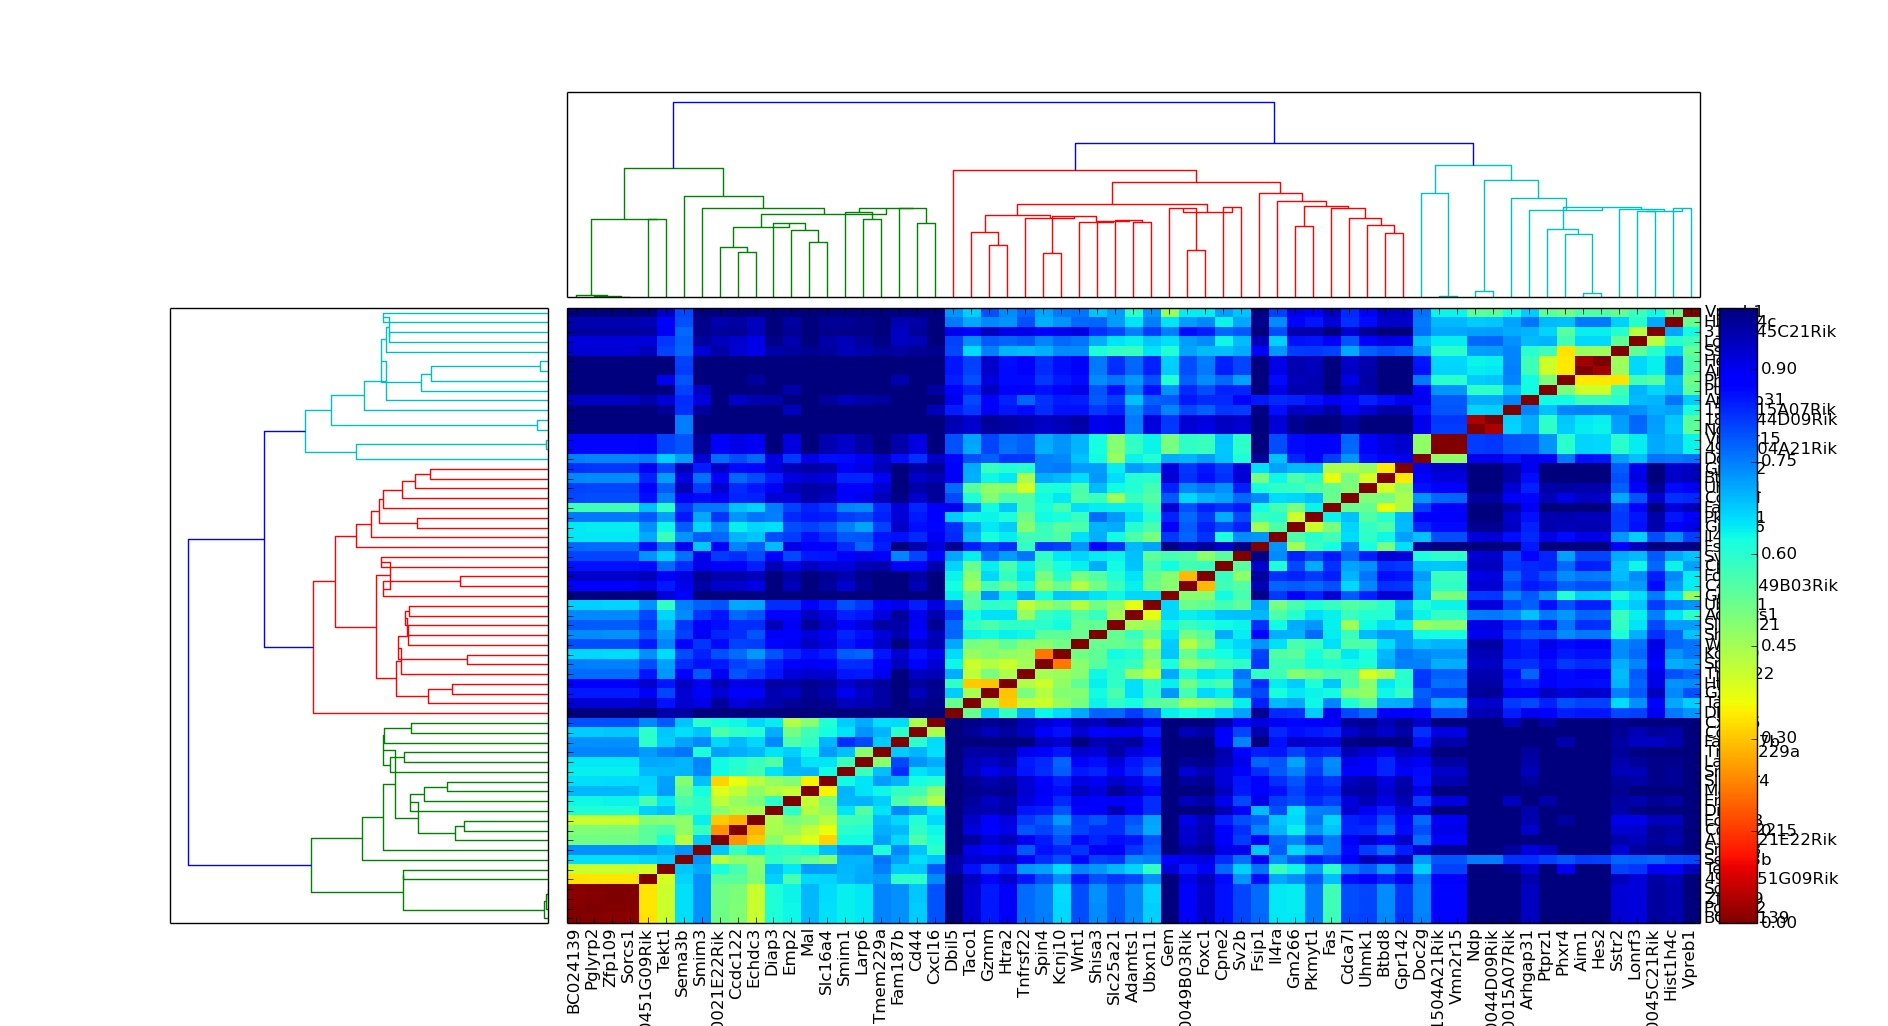
\includegraphics[width = 120mm]{figs/f25.jpg}    
\end{center}
    
\texttt{SCTDA.RootedGraph.candidate\_supopoulations()} computes the adjacency and
Jensen-Shannon matrices of the genes in the list and looks for pairs of genes that
have both high adjacency and high Jensen-Shannon distance. A threshold
in this 2-dimensional space is set using the option \texttt{thres}, taking values between 0
and 1. The first plot produced by
\texttt{SCTDA.RootedGraph.candidate\_supopoulations()} displays the distribution
in this 2-dimensional space of all considered pairs of genes, with pairs passing
the threshold marked in red. Genes that appear in pairs of genes that
pass the threshold are then clustered using hierarchical clustering and
Jensen-Shannon distance. In our particular example, three potential
types/stages of progenitor motor neurons are detected. At the end of
this process, \texttt{SCTDA.RootedGraph.candidate\_supopoulations()} returns a
list with the genes in each of the clusters defining potential cell
sub-populations,

    % Make sure that atleast 4 lines are below the HR
    \needspace{4\baselineskip}

    
        \vspace{8pt}
        \makebox[0.1\linewidth]{\smaller\hfill\tt\color{nbframe-in-prompt}In\hspace{4pt}{[}38{]}:\hspace{4pt}}\\*
        \vspace{-2.1\baselineskip}
        \begin{ColorVerbatim}
            \vspace{-0.2\baselineskip}
            \begin{Verbatim}[commandchars=\\\{\}]
\PY{k}{print} \PY{n}{u}
\end{Verbatim}

            
                \vspace{-0.2\baselineskip}
            
        \end{ColorVerbatim}
    

    

        % If the first block is an image, minipage the image.  Else
        % request a certain amount of space for the input text.
        \needspace{4\baselineskip}
        
        

            % Add document contents.
            
                \begin{InvisibleVerbatim}
\begin{alltt}{\small[['4921504A21Rik', 'Vmn2r15', 'Doc2g', 'Ndp', '1810044D09Rik', 'Aim1', 'Hes2', 
'Phxr4', 'Ptprz1', 'Lonrf3', '3110045C21Rik', 'Hist1h4c', 'Vpreb1', 'Sstr2', 
'Arhgap31', '1500015A07Rik'], ['Gzmm', 'Htra2', 'Taco1', 'Spin4', 'Kcnj10', 
'Adamts1', 'Ubxn11', 'Slc25a21', 'Shisa3', 'Wnt1', 'Tnfrsf22', 'C430049B03Rik', 
'Foxc1', 'Gem', 'Cpne2', 'Sv2b', 'Gm266', 'Pkmyt1', 'Btbd8', 'Gpr142', 'Uhmk1', 
'Cdca7l', 'Fas', 'Il4ra', 'Fsip1', 'Dbil5'], ['Zfp109', 'Sorcs1', 'Pglyrp2', 
'BC024139', '4930451G09Rik', 'Tekt1', 'Ccdc122', 'Echdc3','A330021E22Rik', 
'Mal', 'Slc16a4', 'Emp2', 'Diap3', 'Larp6', 'Tmem229a', 'Smim1', 'Cd44', 
'Cxcl16', 'Fam187b', 'Smim3', 'Sema3b']]
}
\end{alltt}

            \end{InvisibleVerbatim}
            
        
    


    % Make sure that atleast 4 lines are below the HR
    \needspace{4\baselineskip}

    
        \vspace{8pt}
        \makebox[0.1\linewidth]{\smaller\hfill\tt\color{nbframe-in-prompt}In\hspace{4pt}{[}39{]}:\hspace{4pt}}\\*
        \vspace{-2.1\baselineskip}
        \begin{ColorVerbatim}
            \vspace{-0.2\baselineskip}
            \begin{Verbatim}[commandchars=\\\{\}]
\PY{n}{c}\PY{o}{.}\PY{n}{draw}\PY{p}{(}\PY{n}{u}\PY{p}{)}\PY{p}{;}
\end{Verbatim}

            
                \vspace{-0.2\baselineskip}
            
        \end{ColorVerbatim}
    
\begin{center}
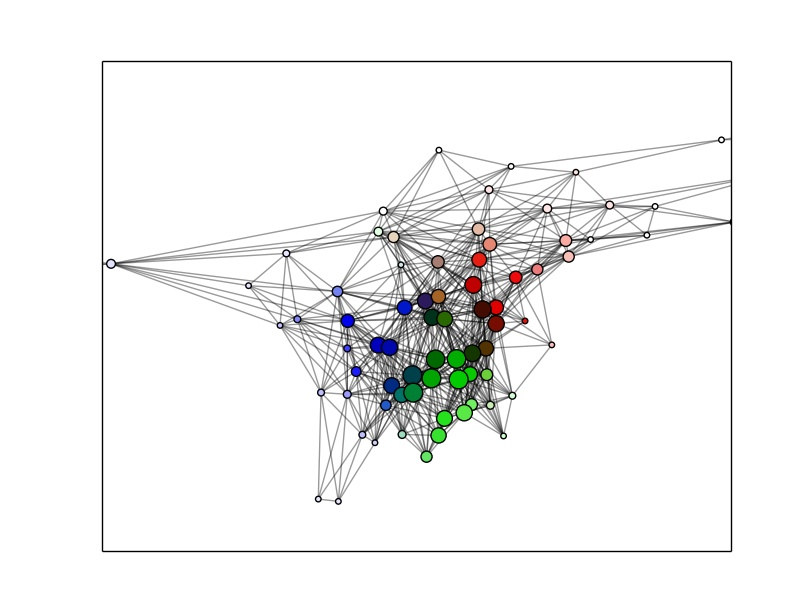
\includegraphics[width = 110mm]{figs/f26.jpg}    
\end{center}

        

        \renewcommand{\indexname}{Index}
        \printindex

    % End of document
    \begin{thebibliography}{99}
    \bibitem{ref1} Rizvi, A., Camara, P. G., Kandror, E., Rabadan, R. and Maniatis, T., \emph{Title of paper}. In preparation.
    \end{thebibliography}
    \end{document}


